%!TEX root = ../dissertation.tex
\begin{savequote}[75mm]
Every question has a proper answer. Every soul has a proper place.
%\qauthor{Tony.}
\end{savequote}

\chapter{Systematics}
\label{sec:systematics}


%%%%%%%%%%%%%%%%%%%%%%%%%%%%%%%%%%%%%%%%%%%%%%%%%%%%%%%%%%%%%%%%%%%%%%%
%%%%%%%%%%%%%%%%%%%%%%%%%%%%%%%%%%%%%%%%%%%%%%%%%%%%%%%%%%%%%%%%%%%%%%%
\section{Overview}
\label{sec:systematics-overview}
\paragraph{}
This analysis is statistically limited.
The largest uncertainties for signal processes are from $b$-tagging efficiency corrections and jet mass resolution.
The major background, QCD, is estimated with the data-driven method. 
Therefore, detector modeling uncertainties have very small impacts on the background estimation.
The largest background estimation uncertainty comes from the differences between data and prediction in the control regions.
The total uncertainties for the boosted analysis will decrease with higher integrated luminosity in the future.

\paragraph{}
The signal acceptance is affected by theoretical uncertainties described in section~\ref{sec:boosted-systematics-theory}.
These are renormalization and factorization scales uncertainties, PDF uncertainties, and initial state radiation (ISR) and final state radiation (FSR) uncertainties.
The ISR and FSR variations are the largest theoretical uncertainties.
The uncertainty on the expected signal yield is typically below $10\%$ but can increase to $23\%$, depending on the signal mass.

\paragraph{}
Detector modeling uncertainties are evaluated in section~\ref{sec:boosted-systematics-detector}.
They include $b$-tagging efficiencies, jet energy scale (JES), jet energy resolution (JER), and jet mass resolution (JMR).
These uncertainties can change both the shape and normalization of the signal and \ttbar~ distributions.

\paragraph{}
A statistical uncertainty on the value of \muqcd~ and \alphatt~ for the $4b$, $3b$, and $2bs$ signal regions is determined from the fitting procedure described in section~\ref{sec:ttbarnorm}.
Two uncertainties are calculated from the covariance matrix of the normalization fit, which are then applied to the background predictions.
Correlations between \alphatt~ and \muqcd~ are fully retained.
%Specifically, \muqcd~ and \alphatt~ can be rewritten as a vector, $a = (a_1,\ a_2)$, and the covariance matrix of $a$ is $C$ where $C_{ij} = Cov(a_i,\ a_j)$, then $C$ can be decomposed as:
% \begin{equation}
% C = U \Lambda U^{T}
% \end{equation}
% where $U$ is a unitary matrix whose columns are the eigenvectors of $C$ and $\Lambda = Diag(\Lambda_{1},\Lambda_{2})$ is a real diagonal matrix whose entries are the eigenvalues of $C$.
% The vector $a$ can be projected along the direction of the eigenvectors, i.e. $a \to a^{\prime} = U^{T}a$, then the resulting eigenvalues are uncorrelated because $C \to C^{\prime} = U^{T} C U = \Lambda$.  
% Therefore, the values of $a^{\prime}_{i}$ can be varied independently by $\pm \Lambda_i$ to propagate the uncertainty.  
% To return to the original space of $a$, the system is rotated back with the $U$ matrix.

\paragraph{}
The background modeling uncertainties are derived from the difference between data and prediction in the control regions.
Both the normalization and shape uncertainties in \mtwoJ~ are considered, as discussed in sections~\ref{sec:non-closure-mu-qcd} and ~\ref{sec:unc-shape-qcd-in-sr}. 
The size and shape of sideband and control regions are varied to ensure the uncertainty estimations are robust.

\paragraph{}
The total uncertainties are summarized in section~\ref{sec:boosted-systematics-numbers}.
A validation of these uncertainty estimations are shown in Appendix~\ref{app:appendixZZ}.
Additional uncertainties will be discussed in the Appendix~\ref{app:appendixSys}. 
They include the \ttbar~ theoretical uncertainties, the shape uncertainty of the \ttbar~ prediction in the $3/4b$ signal regions, and the uncertainty from the smoothing function fit range and functional form.

%%%%%%%%%%%%%%%%%%%%%%%%%%%%%%%%%%%%%%%%%%%%%%%%%%%%%%%%%%%%%%%%%%%%%%%
%%%%%%%%%%%%%%%%%%%%%%%%%%%%%%%%%%%%%%%%%%%%%%%%%%%%%%%%%%%%%%%%%%%%%%%
\section{Theoretical uncertainties}
\label{sec:boosted-systematics-theory}
\paragraph{}
The theoretical uncertainties on the acceptance times efficiency ($A\times\varepsilon$) are evaluated by analysis of specially-generated, particle-level signal samples. 
The generation of these samples follows the configuration of the baseline samples, but with modifications to probe the following theoretical uncertainties: uncertainties in the parton density functions, uncertainties due to missing higher order terms in the matrix elements, and uncertainties in the modeling of the underlying event (including multi-parton interactions), of hadronic showers, and of initial and final state radiation.

\paragraph{}
To evaluate the potential effect of missing higher order terms in the matrix element, the renormalization and factorization scales used in the signal generation are varied by both $0.5$ and $2$ for the signals.
The largest difference in signal yield from the default scales is taken as the uncertainty.

\paragraph{}
Uncertainties due to modeling of the parton shower and the underlying event are evaluated by varying the MC generator listed in section~\ref{sec:MC-sig}. 
For the \Grav~ samples, \pythia 8 is switched to Herwig++, while for the scalar and non-resonant signals Herwig++ is switched to \pythia 8.

\paragraph{}
PDF uncertainties are evaluated using the PDF4LHC15\_nlo\_mc set, which combines CT14, MMHT14 and NNPDF3.0 PDF sets \cite{0954-3899-43-2-023001}. 
The uncertainty is evaluated by calculating the acceptance for each PDF set. 
The standard deviation of these acceptance values is taken as the PDF uncertainty.
%For each mass point the distribution of these ratio is compatible with a Gaussian centered on one.
The uncertainty in acceptance due to PDF is less than $\pm1\%$ across the full mass range considered for the analysis.

\paragraph{}
The theoretical uncertainties are implemented in the final statistical analysis as normalization uncertainties on the signals, with the value taken from a polynomial fit of the cross section and the mass of the signal.
This fit smooths out statistical fluctuations and allows interpolation between the generated signal masses.


%%%%%%%%%%%%%%%%%%%%%%%%%%%%%%%%%%%%%%%%%%%%%%%%%%%%%%%%%%%%%%%%%%%%%%%
%%%%%%%%%%%%%%%%%%%%%%%%%%%%%%%%%%%%%%%%%%%%%%%%%%%%%%%%%%%%%%%%%%%%%%%
\section{Detector and reconstruction uncertainties}
\label{sec:boosted-systematics-detector}
\subsection{Luminosity uncertainty} 
\paragraph{}
The uncertainty in the integrated luminosity of the combined 2015 and 2016 datasets is $36.1\,fb^{-1}\pm2.1$\%~\cite{LumiCiteUP}.
This uncertainty is applicable to the backgrounds with normalizations determined from simulation, and further propagated to the QCD prediction through the data-driven background estimation procedure.
This uncertainty is also applied to the signal normalization prediction.
It has a small impact on this analysis. 

\subsection{Large-\R jet resolution and scale uncertainties} 
\paragraph{}
There are uncertainties on the large-\R jets energy scale (JES) and energy resolution (JER), as well as the mass scale (JMS) and mass resolution (JMR).
The uncertainties on the JES and JMS are derived in situ from 13 \TeV~ $pp$ collisions using techniques described in Ref.~\cite{JetMassAndSubstructure}. 
Discrepancies in jet four-momenta observed between data and MC are assigned as uncertainties on the energy/mass scales of the jet.
%The uncertainties are only correlated between energy and mass.

\paragraph{}
The uncertainties on the jet mass resolutions are estimated by applying a Gaussian smearing.
For each signal mass point, the large-\R trimmed jet mass is smeared such that the intrinsic resolution is increased by 20\%. 
For jet energy resolution, the large-\R jet's momentum is smeared with an absolute $2\%$ uncertainty. 
The nominal MC mass resolution ($\sigma_{M}$) for every signal mass is determined by fitting the $M_\text{JJ} / M_\text{truth}$ distribution before the final $X_{hh}$ cut with a Gaussian function.


\subsection{$b$-tagging uncertainties}
\label{sec:b-tagging-unc}
\paragraph{}
Calibrations, or correction factors per \pt~ bin, for the $b$-tagging efficiency of $R=0.2$ track jets have been derived using \ttbar~ events in data and simulation, as described in Ref~\cite{Aad:2015ydr, ATL-COM-PHYS-2015-009, ATL-COM-PHYS-2015-1323}.
The calibrations are applied to the signal and \ttbar~ simulations, for better data and simulation agreement.  
The calibrations also include uncertainties which modify the $b$-tagging efficiency and thus modify the signal or \ttbar~ acceptances.
For $b$-jets with \pt~$> 300$~\GeV, systematic uncertainties in tagging calibrations are extrapolated with simulations and are consequently larger.
These calibration uncertainties are propagated through the full selections.
The $b$-tagging uncertainty changes the signal yield by $30\%$ and the \ttbar~ yield by $12\%$, depending on the $b$-tagging channel.

\paragraph{}
A significant reduction of $b$-tagging systematic uncertainty for resonant signals in the $3b$ channel is observed. 
This is because in the $3b$ channel, there may exist one not $b$-tagged jet, or anti-$b$-tagged jet.
When a $b$-tagged jet is calibrated with a scale factor $w_{sf}$ with uncertainties $\Delta w_{sf}$, any change in $b$-tagging efficiency must be corrected in the opposite direction for the anti-$b$-tagged jets in order to ensure that the total number of events is fixed. 
The anti-$b$-tagging calibration scale factor is defined in Equation~\ref{eqn:antisf}:
\begin{equation}
\label{eqn:antisf}
\Delta  w_{sf}^{anti} = (1 - \Delta  w_{sf} \epsilon_{b}) / (1 - \epsilon_{b})
\end{equation}
where $\epsilon_{b}$ is the tagging efficiency.
In the $4b$ channel, $(\Delta w_{sf})^4$ is applied on the MC event weight as the uncertainty.
In the $3b$ channel, $(\Delta w_{sf})^3 \Delta  w_{sf}^{anti} $ is the uncertainty.
This anti-correlation reduces the $b$-tagging uncertainty on the $3b$ signal region. 
In the $2bs$ channel, $(\Delta w_{sf})^2 (\Delta  w_{sf}^{anti})^2 $ is the uncertainty.
This makes the $b$-tagging uncertainty larger in the $2bs$ channel than the $3b$ channel.

\paragraph{}
This feature is justified in Figure~\ref{fig:signal_bsyst_reduction}.
One variation of $b$-tagging scale factor is tested on \Grav~ simulations.
In the $4b$ plot, no $\Delta  w_{sf}^{anti}$ is applied. 
The variation on the signal yield is only due to $\Delta w_{sf}$.
In the $3b$ plot, $\Delta  w_{sf}^{anti}$ is applied. 
This $w_{sf}^{anti}$ reduces the variation from $\Delta w_{sf}$.
In the $2bs$ plot, $(\Delta  w_{sf}^{anti})^2$ is applied. 
This $w_{sf}^{anti}$ further reduces the variation from $\Delta w_{sf}$, causing the signal yield difference increase in comparison with the $3b$ case.

\begin{figure*}[htb!]
\centering
\captionsetup{justification=centering}
    \begin{subfigure}[b]{0.45\textwidth}
        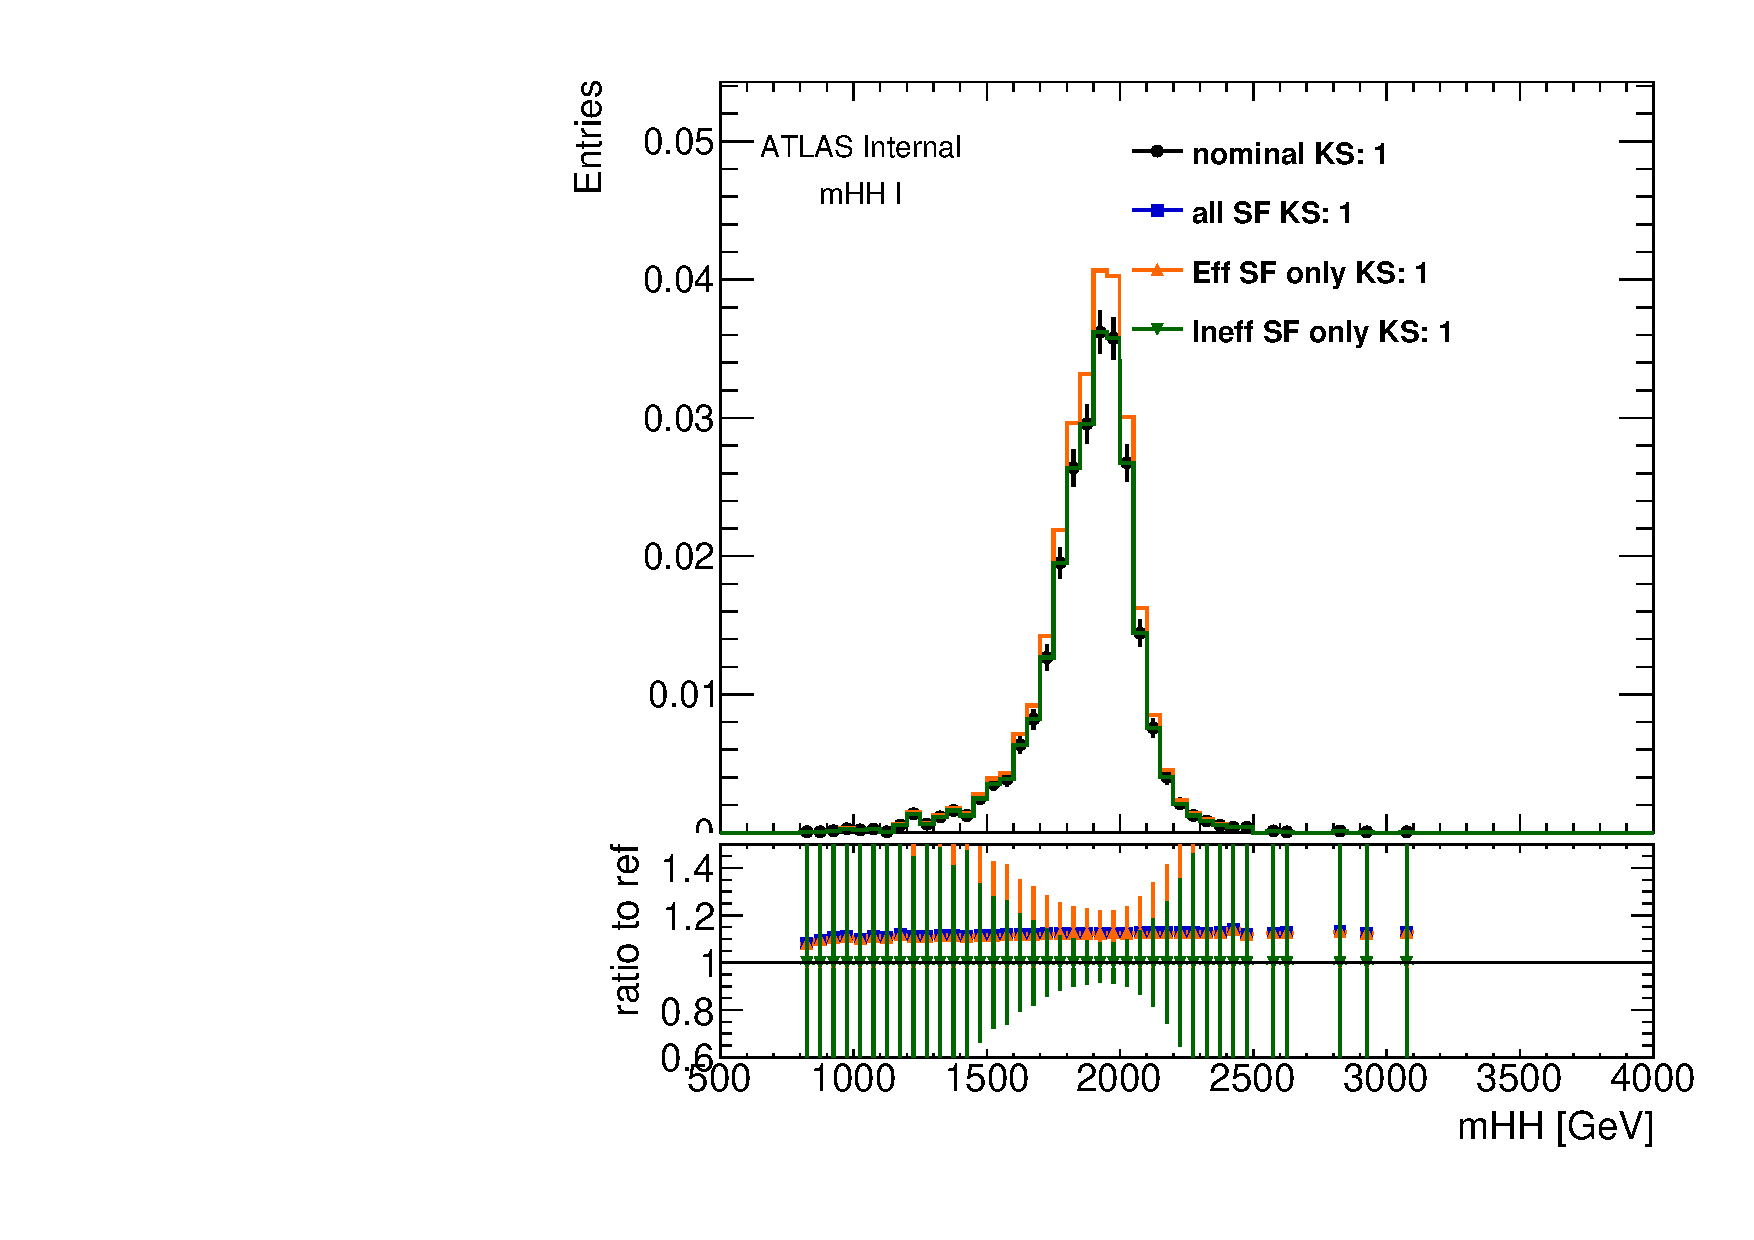
\includegraphics[width=\textwidth,angle=-90]{figures/boosted/AppendixbSF/directcompare_mHH_l_bSF_2000_FT_EFF_Eigen_B_0__1down_FourTag_.pdf}
        \caption{$4b$}
        \label{fig:signal_bsyst_reduction-4b}
    \end{subfigure}
    \quad 
    \begin{subfigure}[b]{0.45\textwidth}
        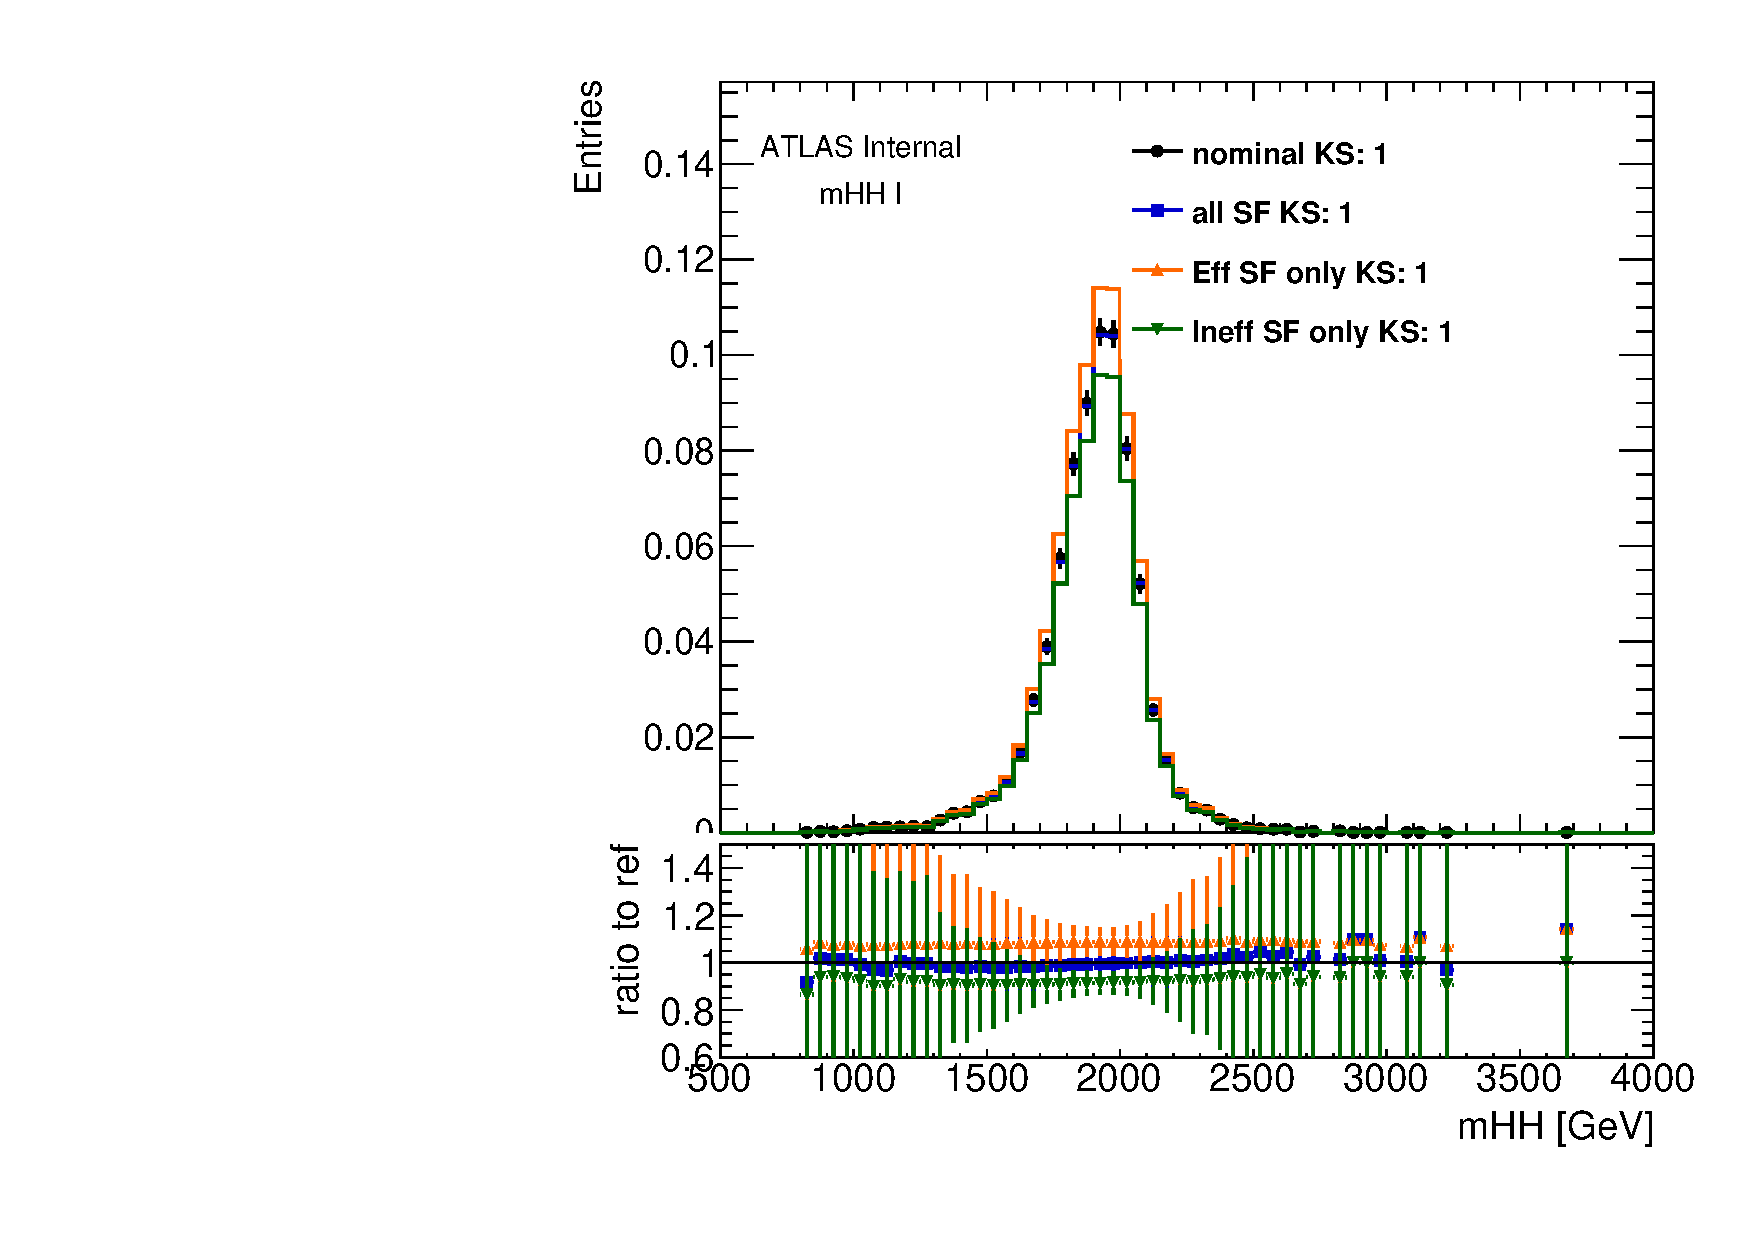
\includegraphics[width=\textwidth,angle=-90]{figures/boosted/AppendixbSF/directcompare_mHH_l_bSF_2000_FT_EFF_Eigen_B_0__1down_ThreeTag_.pdf}
        \caption{$3b$}
        \label{fig:signal_bsyst_reduction-3b}
    \end{subfigure}
    \\
    \begin{subfigure}[b]{0.45\textwidth}
        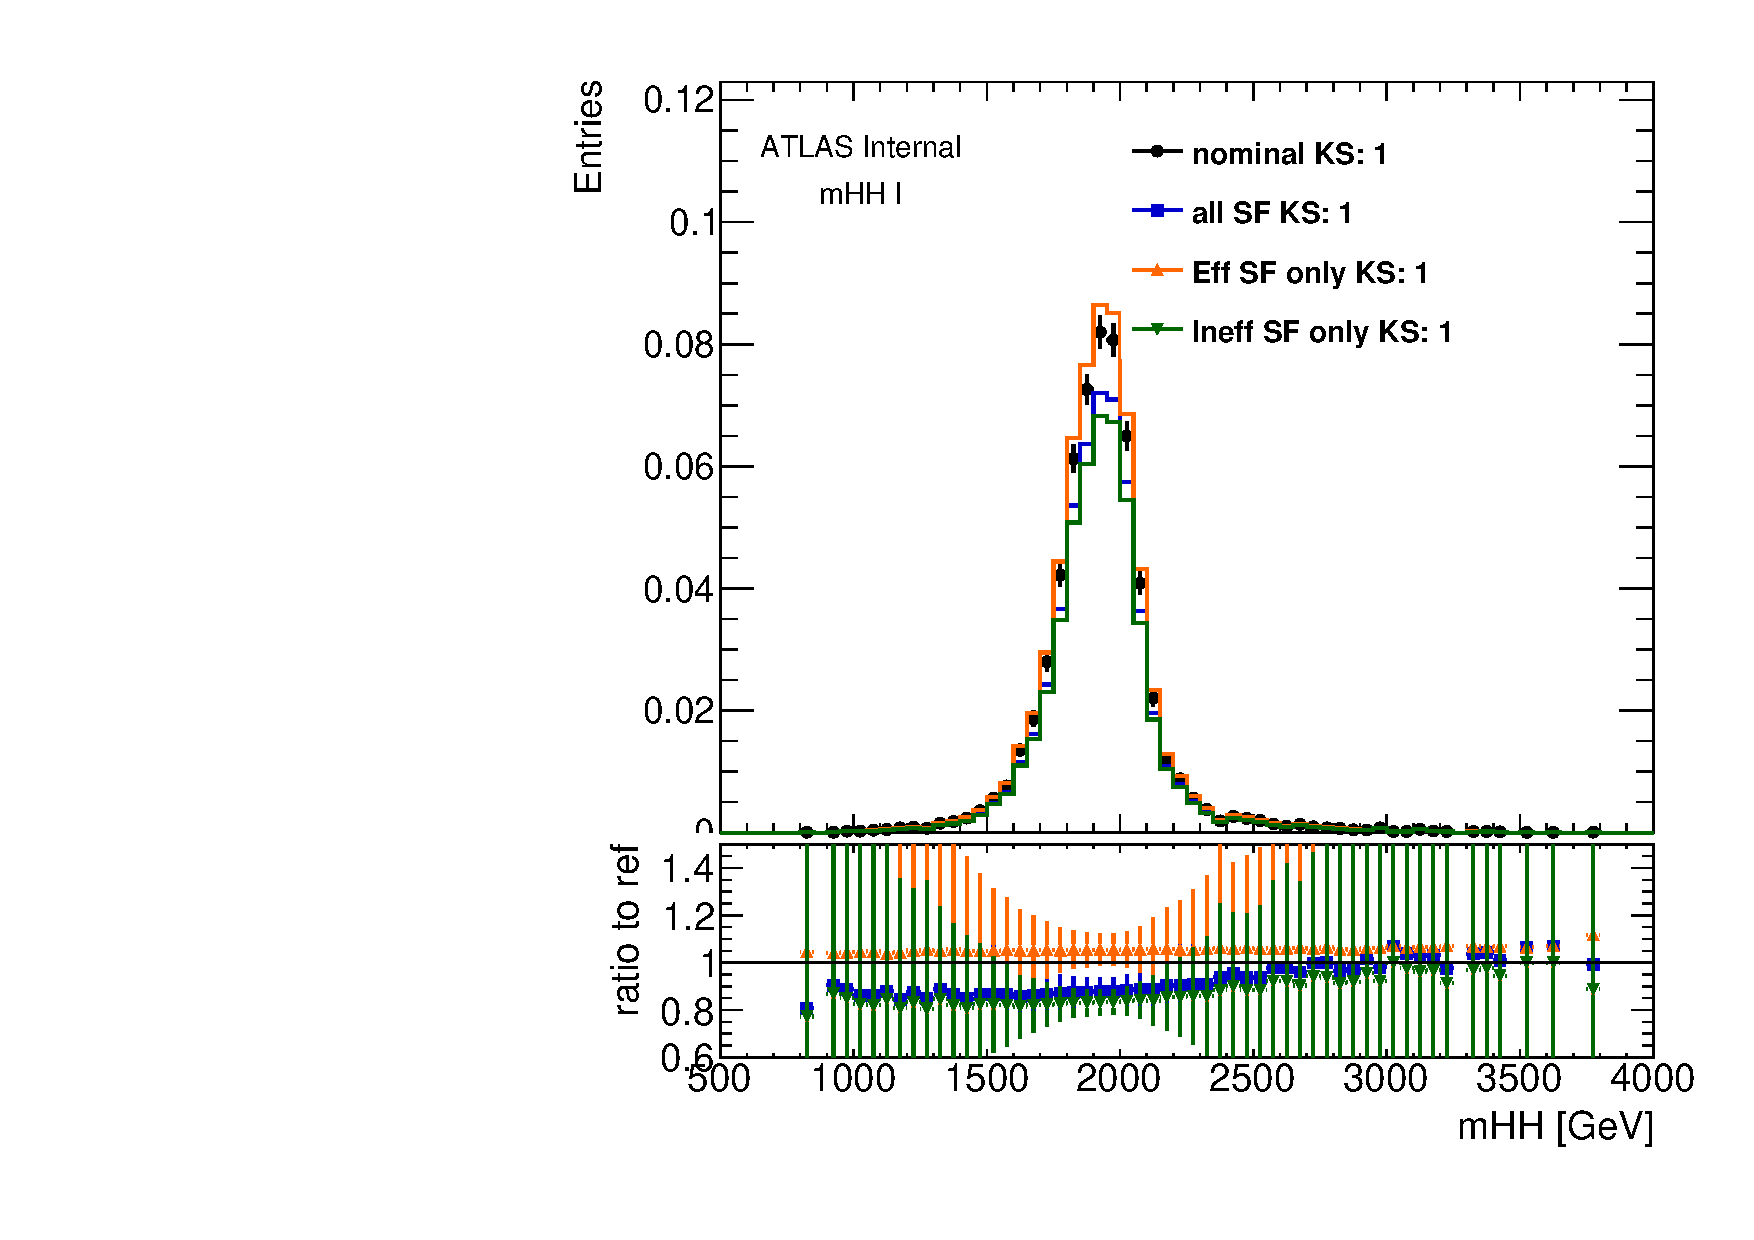
\includegraphics[width=\textwidth,angle=-90]{figures/boosted/AppendixbSF/directcompare_mHH_l_bSF_2000_FT_EFF_Eigen_B_0__1down_TwoTag_split_.pdf}
        \caption{$2bs$}
        \label{fig:signal_bsyst_reduction-2b}
    \end{subfigure}
  \caption{Impact on \mtwoJ~ of the efficiency scale factor $w_{sf}$ and inefficiency scale factor $w_{sf}^{anti}$. The MC is $2$ \TeV~ \Grav~ with $c=1.0$.}
  \label{fig:signal_bsyst_reduction}
\end{figure*}


%%%%%%%%%%%%%%%%%%%%%%%%%%%%%%%%%%%%%%%%%%%%%%%%%%%%%%%%%%%%%%%%%%%%%%%
%%%%%%%%%%%%%%%%%%%%%%%%%%%%%%%%%%%%%%%%%%%%%%%%%%%%%%%%%%%%%%%%%%%%%%%
\section{Background normalization uncertainties}
\label{sec:non-closure-mu-qcd}

\paragraph{}
\muqcd~ estimation is dependent on the choices of sideband region and control region.
Additional sideband and control regions were designed and tested. 
They are further illustrated in Appendix~\ref{app:appendixSysVar} and are listed below:
\begin{itemize}
	\item Low-mass control region: the center position of the circle that defines nominal control region is moved down by $3$ \GeV~ in both leading and sub-leading large-jet mass.
	\item High-mass CR: the center position of the circle that defines nominal control region is moved up by $3$ \GeV~ in both leading and sub-leading large-R jet mass.
	\item Signal-depletion control region (Small CR): the $X_{hh}$ cut that defines signal region is increased to $2.0$ from $1.6$. This variation only affect the control region, while the signal region remains unchanged (i.e. the signal region is still defined by $X_{hh}<1.6$, while the control region is defined with $X_{hh}>2.0$ and $R_{hh}<33$ \GeV).
	\item High-mass sideband region: The signal region and control region remain unchanged, and the center position of the circle that defines nominal SB is moved up by 3 GeV in both the leading and sub-leading large-\R jet mass.
	\item Low-mass sideband region: The signal region and control region remain unchanged, and the center position of the circle that defines nominal SB is moved up by 3 GeV in both the leading and sub-leading large-\R jet mass.
	\item Large sideband region: The signal region and control region remain unchanged, and the sideband region is redefined as $33$ \GeV $< R_{hh}$ and $ R_{hh}^{\text{high}} < 61$ \GeV. 
	\item Small sideband region: The signal region and control region remain unchanged, and the sideband region is redefined as $33$ \GeV $< R_{hh}$ and $ R_{hh}^{\text{high}} < 55$ \GeV.
\end{itemize}

\paragraph{} 
These variations are tested after the full reweighting procedure as described in section~\ref{sec:boosted-reweight}.
The differences between prediction and observed data are summarized in Tables~\ref{tab:Tab_4b_CR_Variations}, \ref{tab:Tab_3b_CR_Variations}, and \ref{tab:Tab_2bs_CR_Variations}.
Based on these differences, the largest differences between the predicted backgrounds and observed data is taken as the uncertainty.
A final $2.9\%$ normalization uncertainty is assigned to the $2bs$ signal region, $4.3\%$ to the $3b$ signal region, and a $12.2\%$ normalization uncertainty is assigned to the $4b$ signal region.

\begin{table}[htb!]
\begin{center}
\caption{Observed data and predictions in $4b$ control region with statistical uncertainties.}
\begin{footnotesize} 
\begin{tabular}{c|c|c|c} 
CR Varations FourTag & Data & Prediction & (Predict - Data)/Data \\ 
\hline\hline 
& & & \\ 
Nominal & 81.0 $\pm$ 9.0 & 76.77 $\pm$ 5.43 & -5.22 $\%$  $\pm$ 17.23 $\%$ \\ 
\hline 
CR High & 76.0 $\pm$ 8.72 & 71.12 $\pm$ 5.41 & -6.43 $\%$  $\pm$ 17.85 $\%$ \\ 
\hline 
CR Low & 91.0 $\pm$ 9.54 & 79.87 $\pm$ 5.45 & -12.2 $\%$  $\pm$ 15.19 $\%$ \\ 
\hline 
CR Small & 58.0 $\pm$ 7.62 & 55.96 $\pm$ 5.35 & -3.52 $\%$  $\pm$ 21.89 $\%$ \\ 
\hline 
SB Large & 81.0 $\pm$ 9.0 & 74.71 $\pm$ 5.4 & -7.76 $\%$  $\pm$ 16.91 $\%$ \\ 
\hline 
SB Small & 81.0 $\pm$ 9.0 & 74.15 $\pm$ 5.38 & -8.45 $\%$  $\pm$ 16.81 $\%$ \\ 
\hline 
SB High & 81.0 $\pm$ 9.0 & 78.72 $\pm$ 5.46 & -2.82 $\%$  $\pm$ 17.54 $\%$ \\ 
\hline 
SB Low & 81.0 $\pm$ 9.0 & 76.51 $\pm$ 5.38 & -5.54 $\%$  $\pm$ 17.14 $\%$ \\ 
& & & \\ 
\hline\hline 
\end{tabular} 
\end{footnotesize} 
\newline 

\label{tab:Tab_4b_CR_Variations}
\end{center}
\end{table}

\begin{table}[htb!]
\begin{center}
\caption{Observed data and predictions in $3b$ control region with statistical uncertainties.}
\begin{footnotesize} 
\begin{tabular}{c|c|c|c} 
CR Varations ThreeTag & Data & Prediction & (Predict - Data)/Data \\ 
\hline\hline 
Nominal & 1553.0 $\pm$ 39.41 & 1587.04 $\pm$ 21.4 & 2.19 $\%$  $\pm$ 3.97 $\%$ \\ 
\hline 
CR High & 1461.0 $\pm$ 38.22 & 1473.89 $\pm$ 20.77 & 0.88 $\%$  $\pm$ 4.06 $\%$ \\ 
\hline 
CR Low & 1628.0 $\pm$ 40.35 & 1697.38 $\pm$ 21.75 & 4.26 $\%$  $\pm$ 3.92 $\%$ \\ 
\hline 
CR Small & 1134.0 $\pm$ 33.67 & 1127.34 $\pm$ 17.66 & -0.59 $\%$  $\pm$ 4.51 $\%$ \\ 
\hline 
SB Large & 1553.0 $\pm$ 39.41 & 1574.23 $\pm$ 21.47 & 1.37 $\%$  $\pm$ 3.95 $\%$ \\ 
\hline 
SB Small & 1553.0 $\pm$ 39.41 & 1601.44 $\pm$ 21.64 & 3.12 $\%$  $\pm$ 4.01 $\%$ \\ 
\hline 
SB High & 1553.0 $\pm$ 39.41 & 1602.74 $\pm$ 21.48 & 3.2 $\%$  $\pm$ 4.0 $\%$ \\ 
\hline 
SB Low & 1553.0 $\pm$ 39.41 & 1576.56 $\pm$ 21.5 & 1.52 $\%$  $\pm$ 3.96 $\%$ \\ 
\hline\hline 
\end{tabular} 
\end{footnotesize} 
\newline 

\label{tab:Tab_3b_CR_Variations}
\end{center}
\end{table}

\begin{table}[htb!]
\begin{center}
\caption{Observed data and predictions in $2bs$ control region with statistical uncertainties.}
\begin{footnotesize} 
\begin{tabular}{c|c|c|c} 
CR Varations TwoTag split & Data & Prediction & (Predict - Data)/Data \\ 
\hline\hline 
& & & \\ 
Nominal & 8486.0 $\pm$ 92.12 & 8332.97 $\pm$ 38.84 & -1.8 $\%$  $\pm$ 1.52 $\%$ \\ 
\hline 
CR High & 8174.0 $\pm$ 90.41 & 7937.59 $\pm$ 39.61 & -2.89 $\%$  $\pm$ 1.56 $\%$ \\ 
\hline 
CR Low & 8907.0 $\pm$ 94.38 & 8800.86 $\pm$ 39.51 & -1.19 $\%$  $\pm$ 1.49 $\%$ \\ 
\hline 
CR Small & 5999.0 $\pm$ 77.45 & 5873.52 $\pm$ 32.31 & -2.09 $\%$  $\pm$ 1.8 $\%$ \\ 
\hline 
SB Large & 8486.0 $\pm$ 92.12 & 8341.7 $\pm$ 38.44 & -1.7 $\%$  $\pm$ 1.52 $\%$ \\ 
\hline 
SB Small & 8486.0 $\pm$ 92.12 & 8333.25 $\pm$ 39.12 & -1.8 $\%$  $\pm$ 1.53 $\%$ \\ 
\hline 
SB High & 8486.0 $\pm$ 92.12 & 8378.14 $\pm$ 38.45 & -1.27 $\%$  $\pm$ 1.52 $\%$ \\ 
\hline 
SB Low & 8486.0 $\pm$ 92.12 & 8356.86 $\pm$ 39.06 & -1.52 $\%$  $\pm$ 1.53 $\%$ \\ 
& & & \\ 
\hline\hline 
\end{tabular} 
\end{footnotesize} 
\newline 

\label{tab:Tab_2bs_CR_Variations}
\end{center}
\end{table}

%%%%%%%%%%%%%%%%%%
\section{Background \mtwoJ~ shape uncertainties}
\label{sec:unc-shape-qcd-in-sr}
\paragraph{}
As shown in Figure~\ref{fig:boosted-cr-mjj}, the \mtwoJ~ shape of the predicted background is in good agreement with the $4b$, $3b$, and $2bs$ data in the control region.
The differences in \mtwoJ~ distributions in the control region are evaluated and used to assign background \mtwoJ~ estimation uncertainties in the signal region. 
First, the predicted and the data distributions in the control region are smoothed.
The smoothing fits and the ratios are shown in Figures~\ref{fig:qcd_shape_fit_44}, ~\ref{fig:qcd_shape_fit_33}, and ~\ref{fig:qcd_shape_fit_22}.
The ratio between the smoothed background \mtwoJ~ predictions and the smoothed $4b/3b/2bs$ data \mtwoJ~ distributions is taken as the shape systematic uncertainty.
This is the black line in Figures~\ref{fig:qcd_shape_fit_44_ratio}, ~\ref{fig:qcd_shape_fit_33_ratio}, and ~\ref{fig:qcd_shape_fit_22_ratio}.
This systematic uncertainty is further split into two parts: \mtwoJ~$< 2000$ \GeV~ and \mtwoJ~$> 2000$ \GeV.
This ensures the low and high mass region post-fit pulls can vary independently.
The QCD background prediction in the signal region is scaled with this ratio while maintaining the same normalization.
The same shape uncertainty is applied for both the \mtwoJ~ and the scaled \mtwoJ~ distribution. 

\begin{figure*}[htb!]
\begin{center}
    \captionsetup{justification=centering}
    \hspace{-3cm}
    \begin{subfigure}[b]{0.33\textwidth}
        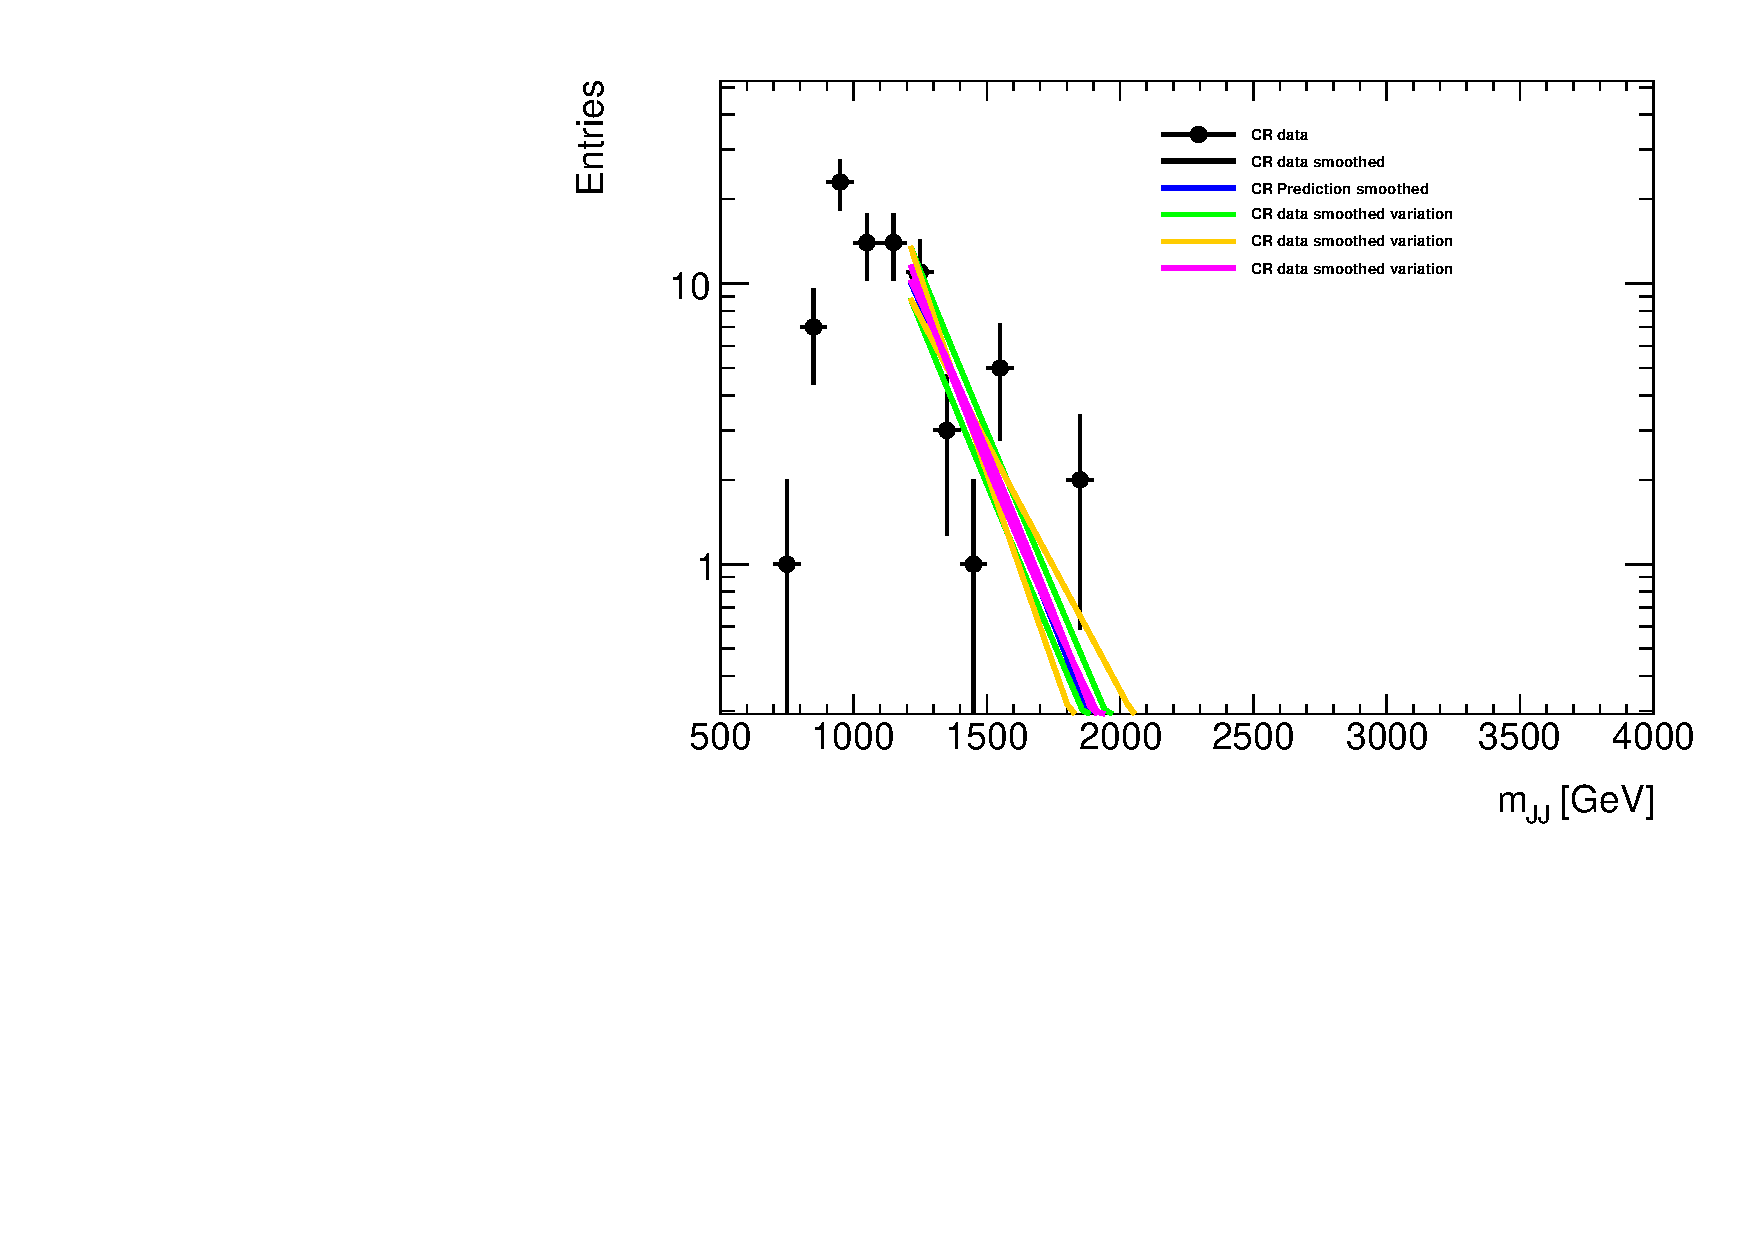
\includegraphics[width=\textwidth,angle=-90]{figures/boosted/Syst_Shape/QCDSysfitSmooth_44.pdf}
        \caption{smoothing fits}
        \label{fig:qcd_shape_fit_44_fit}
    \end{subfigure}
    \quad \quad \quad \quad \quad
    \begin{subfigure}[b]{0.33\textwidth}
        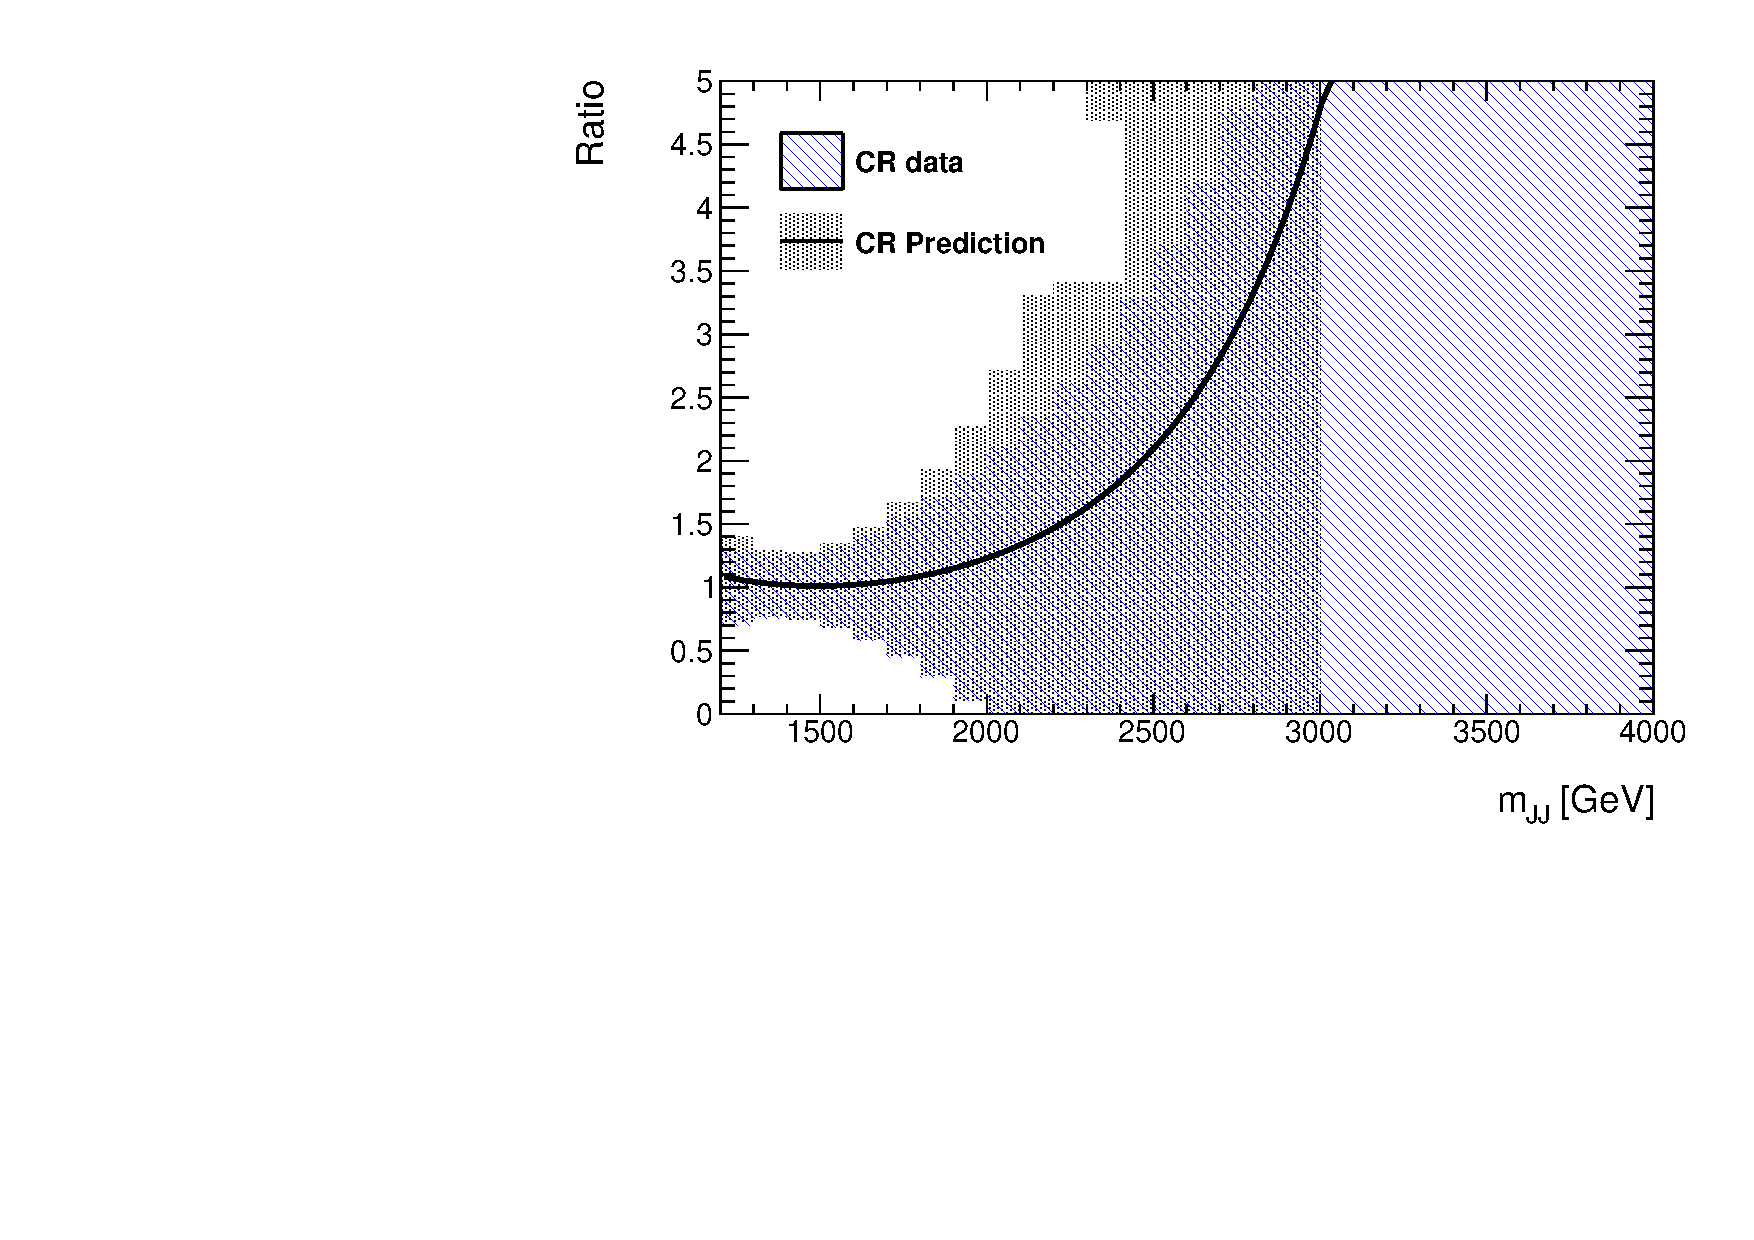
\includegraphics[width=\textwidth,angle=-90]{figures/boosted/Syst_Shape/QCDSysfitSmooth_ratio_44.pdf}
        \caption{ratio of the prediction and data}
        \label{fig:qcd_shape_fit_44_ratio}
    \end{subfigure}
  \caption{\mtwoJ~ smoothing fit and ratio in the $4b$ control region. The uncertainty bands contain the smoothing function parameter variations.}
  \label{fig:qcd_shape_fit_44}
\end{center}
\end{figure*}


\begin{figure*}[htb!]
\begin{center}
    \captionsetup{justification=centering}
    \hspace{-3cm}
    \begin{subfigure}[b]{0.33\textwidth}
        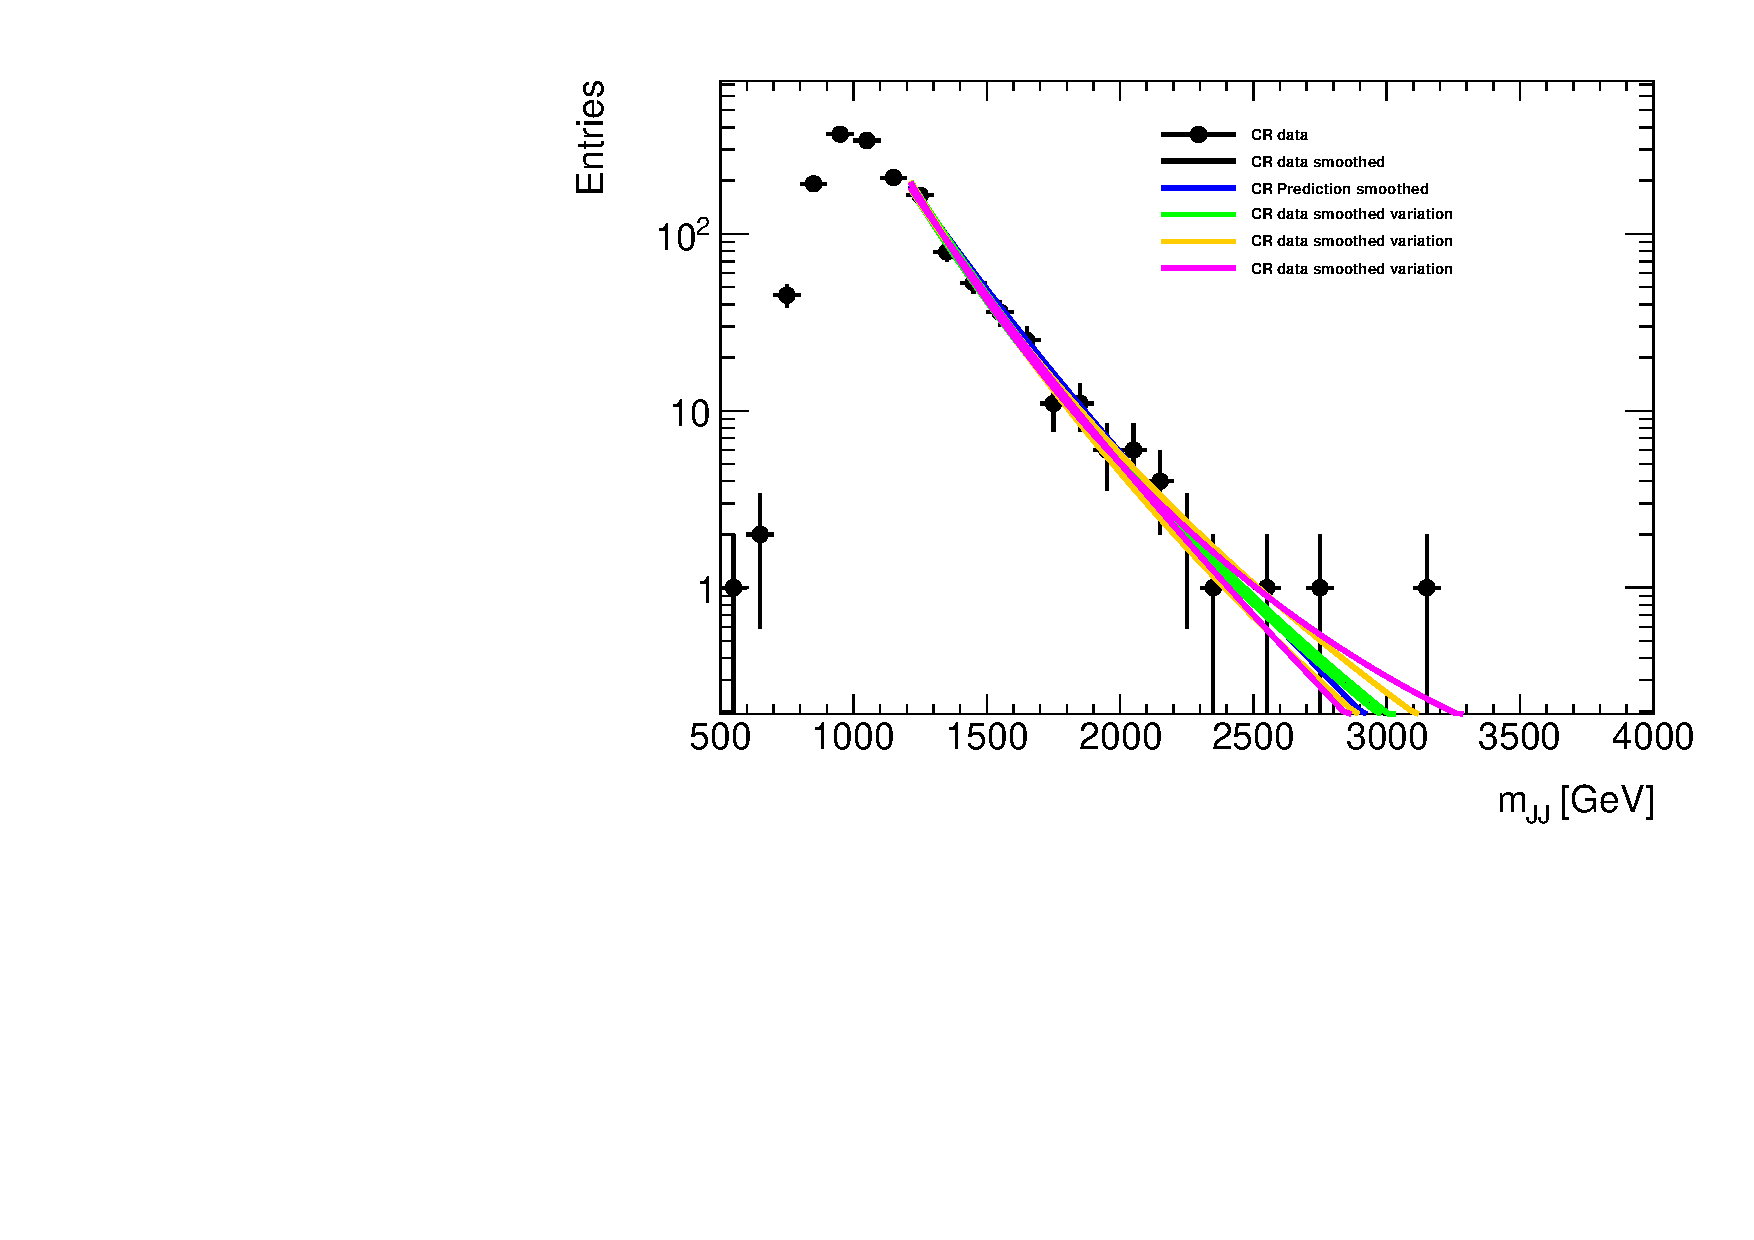
\includegraphics[width=\textwidth,angle=-90]{figures/boosted/Syst_Shape/QCDSysfitSmooth_33.pdf}
        \caption{smoothing fits}
        \label{fig:qcd_shape_fit_33_fit}
    \end{subfigure}
    \quad \quad \quad \quad \quad
    \begin{subfigure}[b]{0.33\textwidth}
        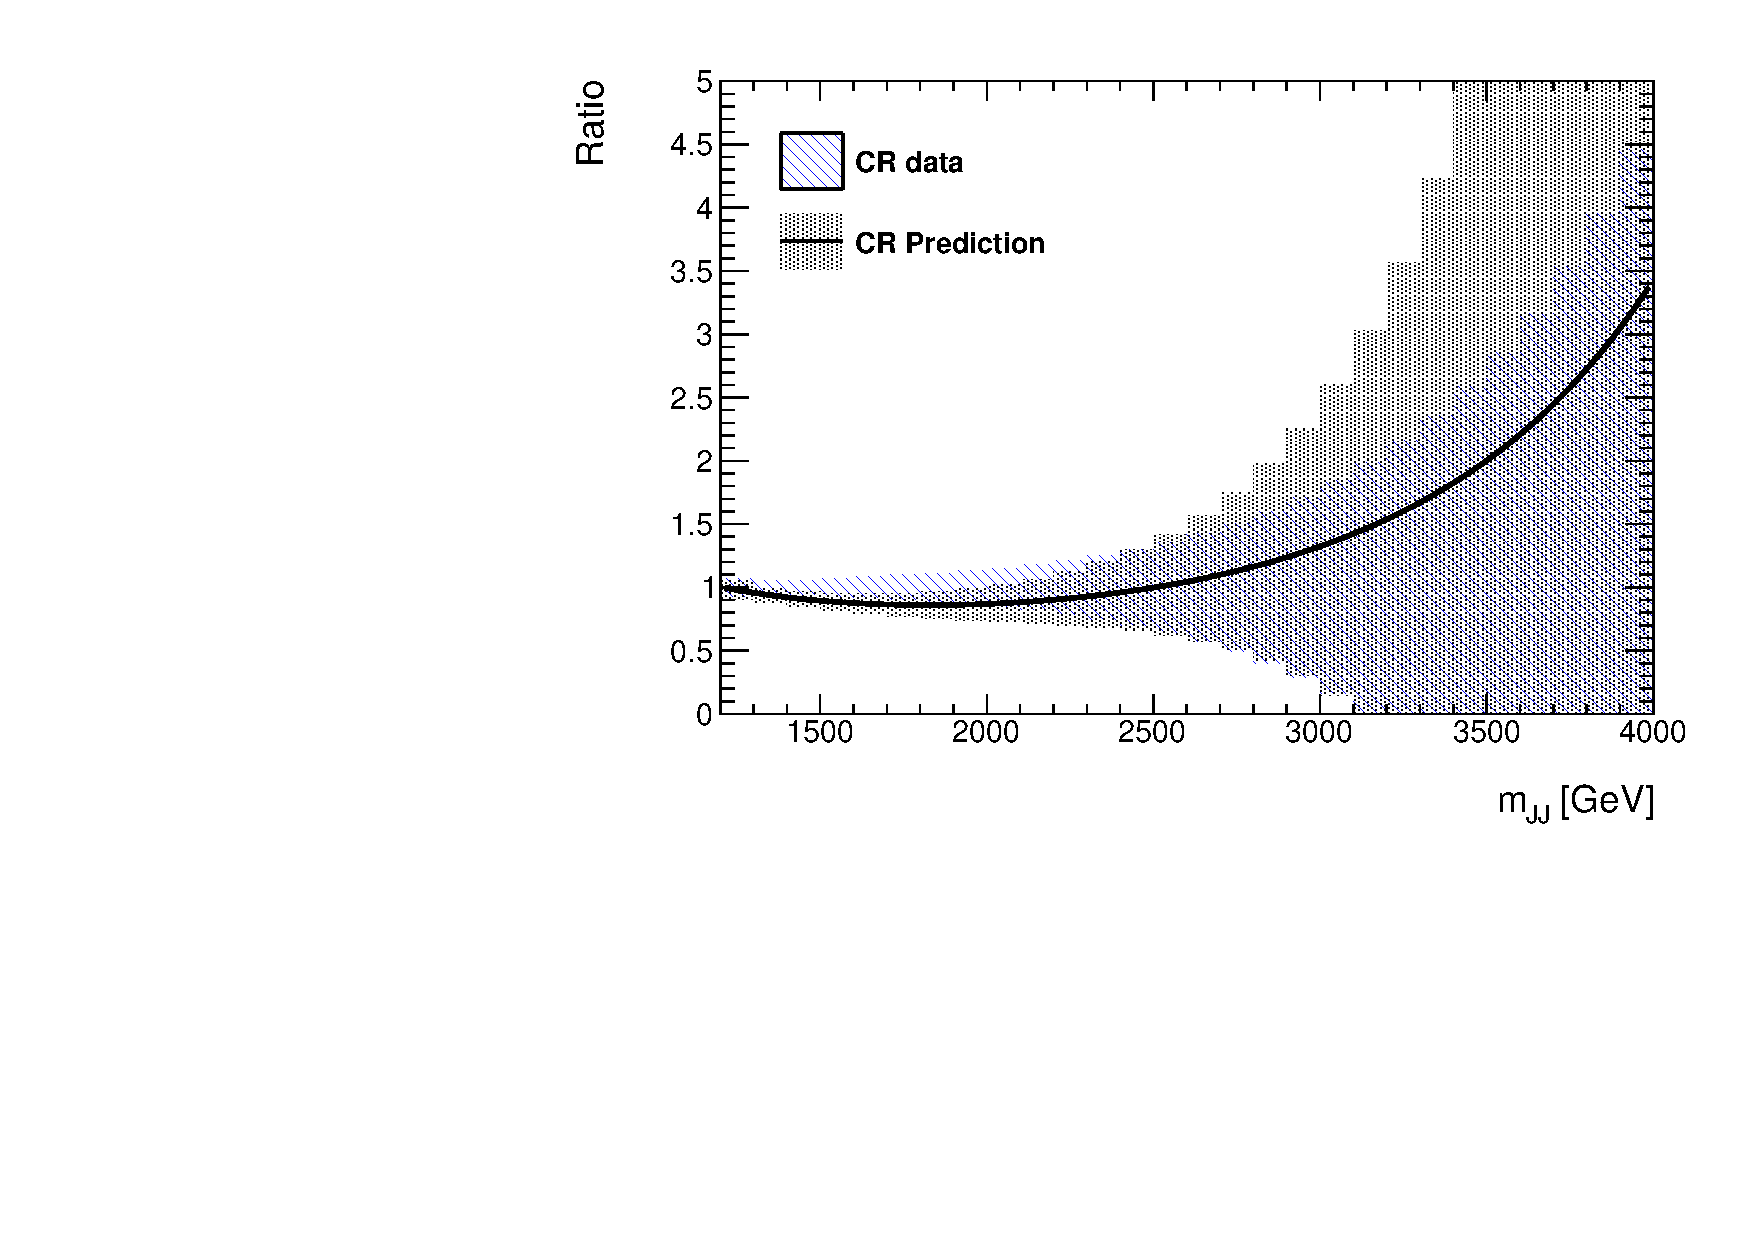
\includegraphics[width=\textwidth,angle=-90]{figures/boosted/Syst_Shape/QCDSysfitSmooth_ratio_33.pdf}
        \caption{ratio of the prediction and data}
        \label{fig:qcd_shape_fit_33_ratio}
    \end{subfigure}
  \caption{\mtwoJ~ smoothing fit and ratio in the $3b$ control region. The uncertainty bands contain the smoothing function parameter variations.}
  \label{fig:qcd_shape_fit_33}
\end{center}
\end{figure*}

\begin{figure*}[htb!]
\begin{center}
    \captionsetup{justification=centering}
    \hspace{-3cm}
    \begin{subfigure}[b]{0.33\textwidth}
        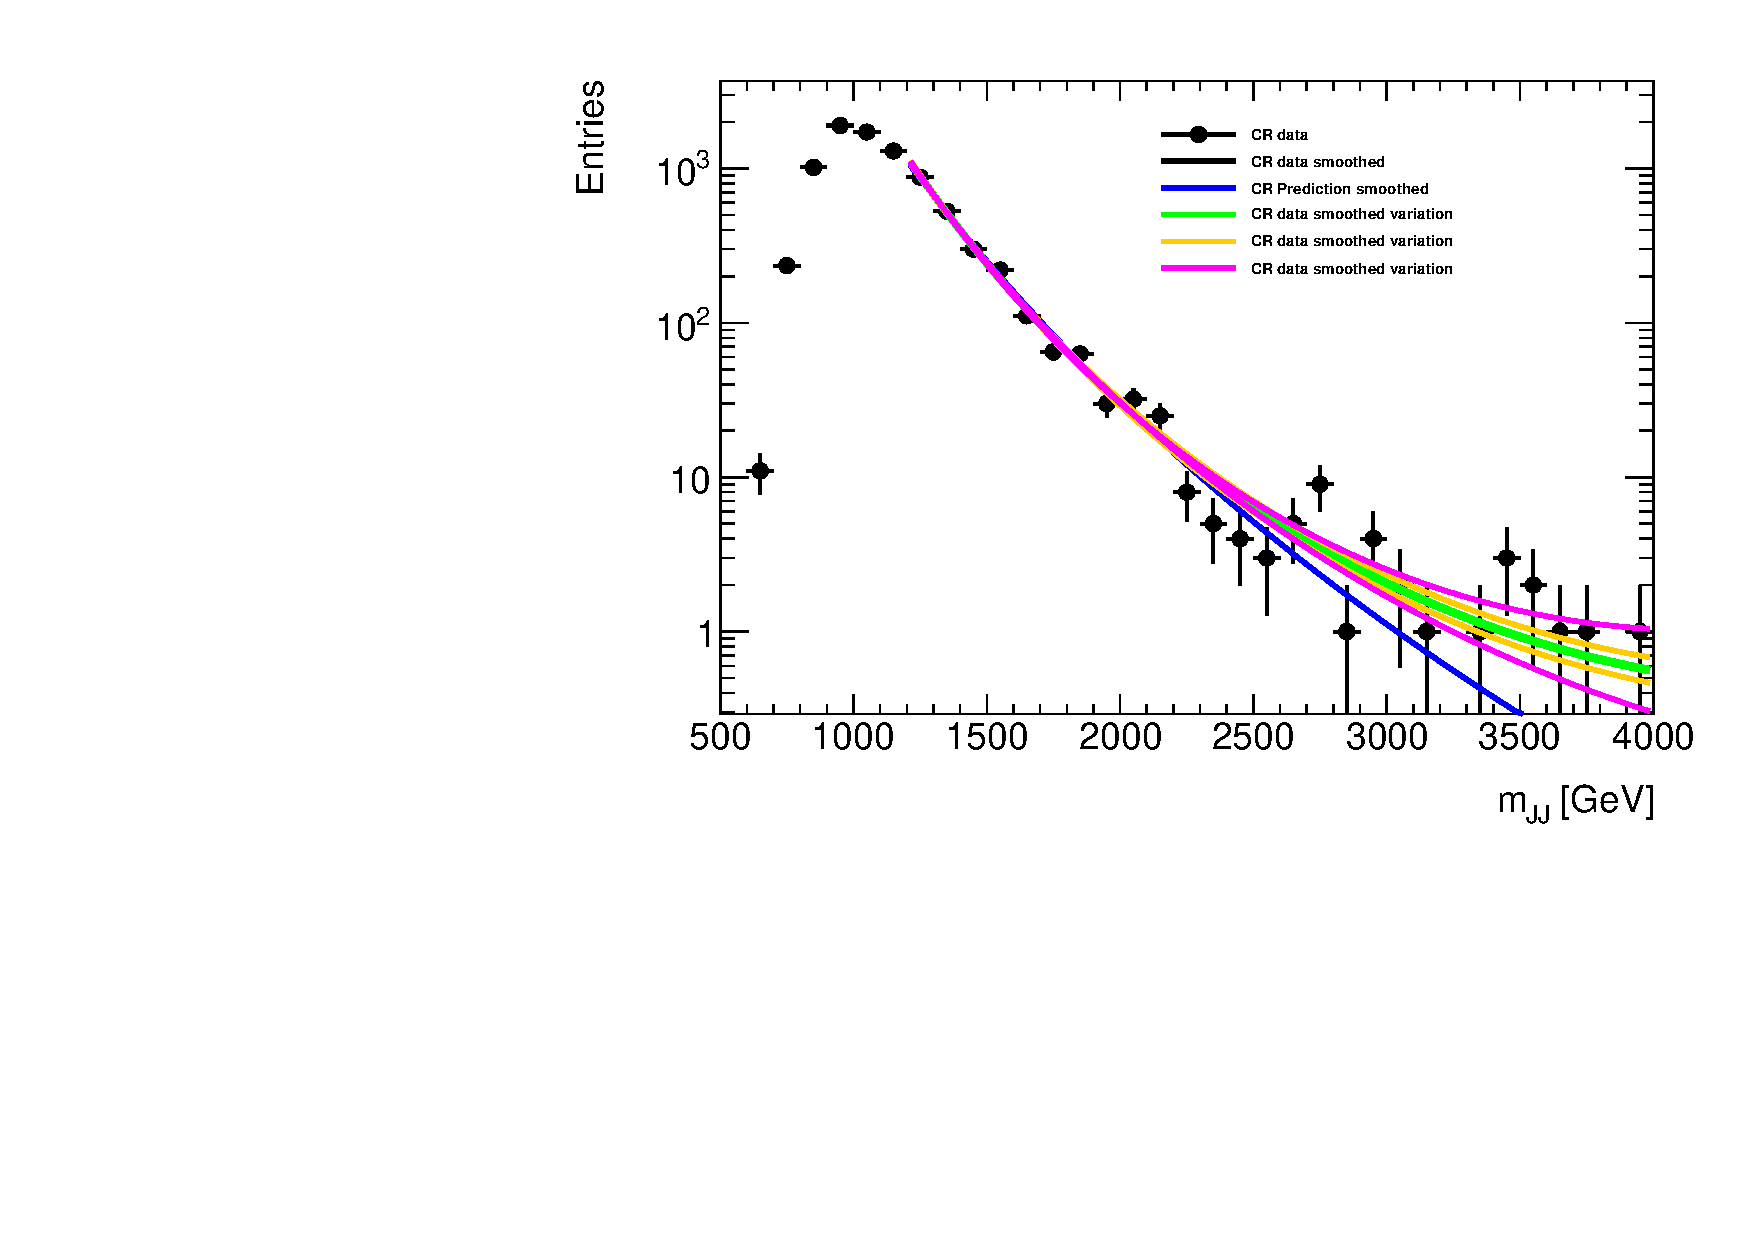
\includegraphics[width=\textwidth,angle=-90]{figures/boosted/Syst_Shape/QCDSysfitSmooth_22.pdf}
        \caption{smoothing fits}
        \label{fig:qcd_shape_fit_22_fit}
    \end{subfigure}
    \quad \quad \quad \quad \quad
    \begin{subfigure}[b]{0.33\textwidth}
        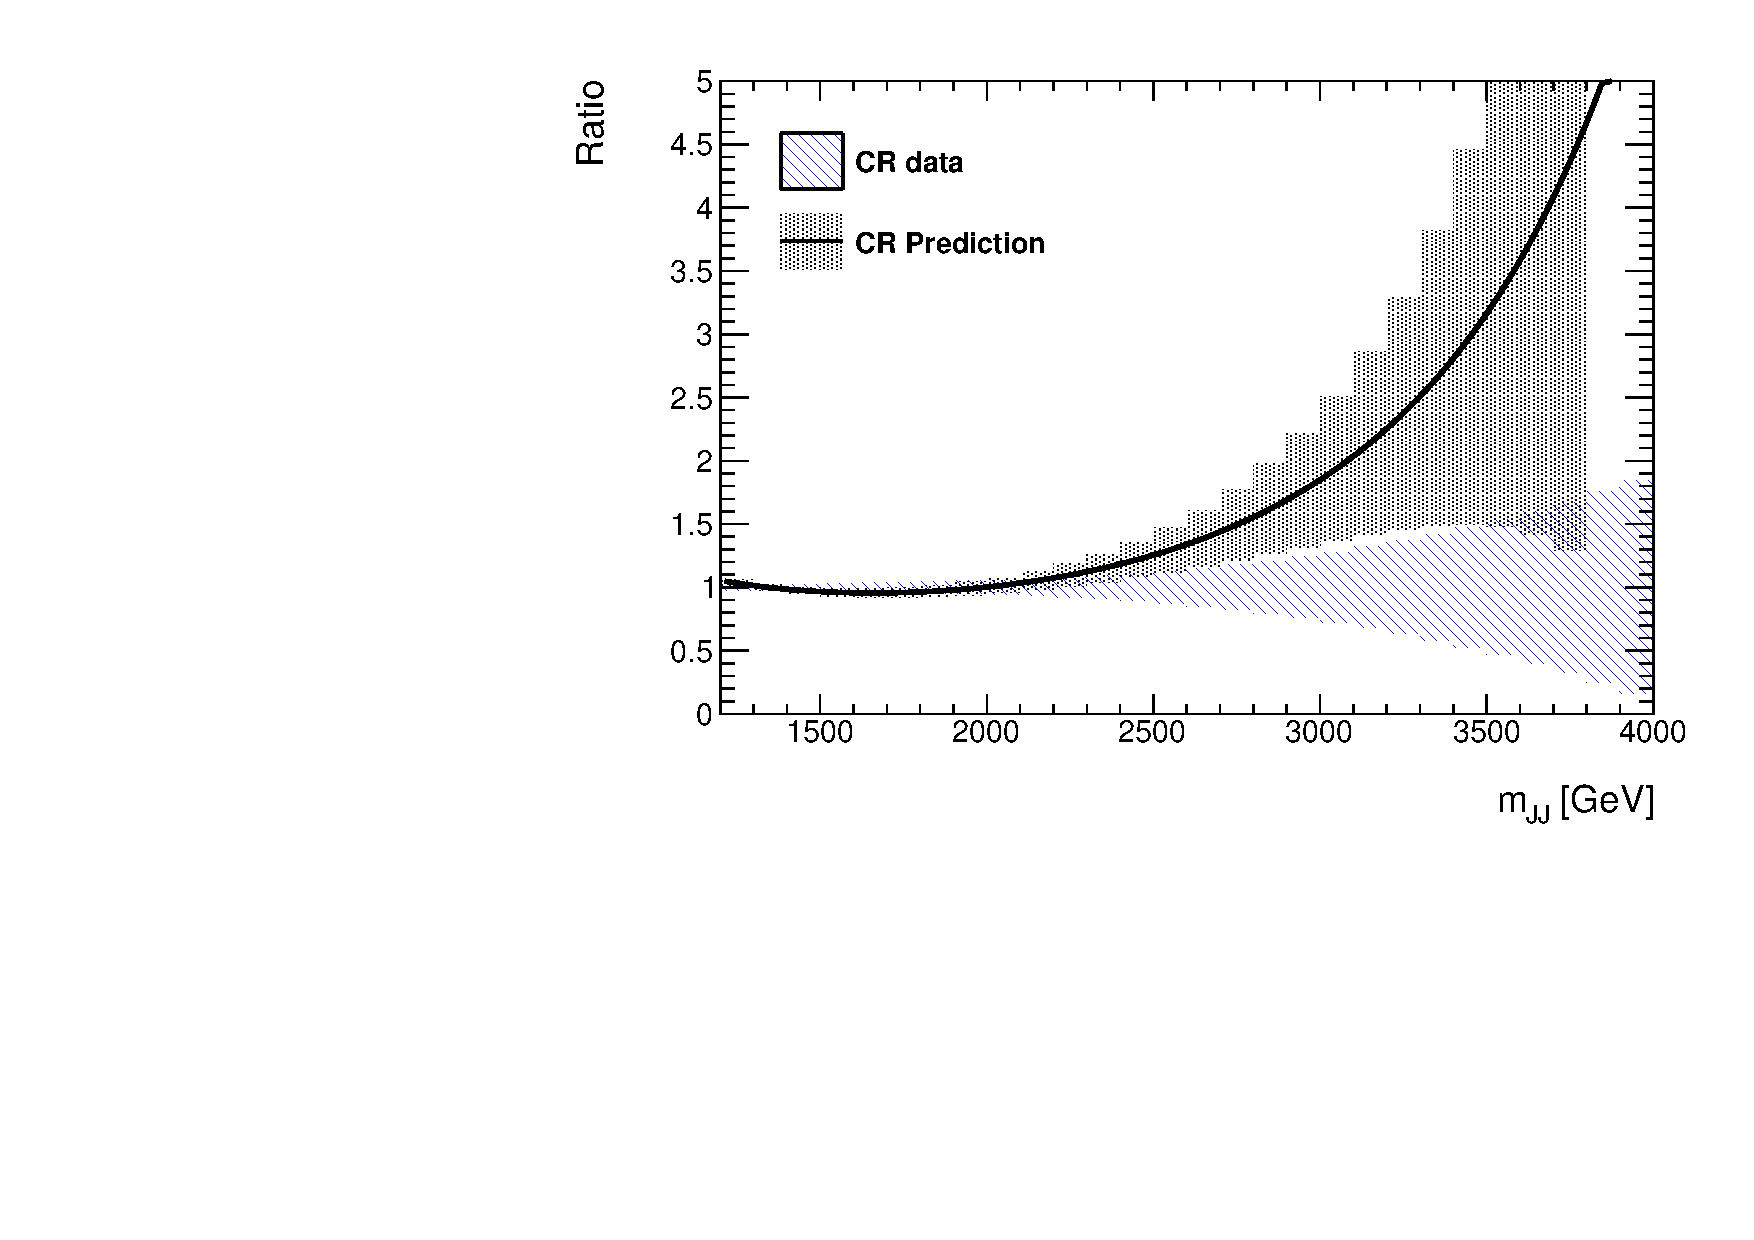
\includegraphics[width=\textwidth,angle=-90]{figures/boosted/Syst_Shape/QCDSysfitSmooth_ratio_22.pdf}
        \caption{ratio of the prediction and data}
        \label{fig:qcd_shape_fit_22_ratio}
    \end{subfigure}
  \caption{\mtwoJ~ smoothing fit and ratio in the $2bs$ control region. The uncertainty bands contain the smoothing function parameter variations.}
  \label{fig:qcd_shape_fit_22}
\end{center}
\end{figure*}



%%%%%%%%%%%%%%%%%%%%%%%%%%%%%%%%%%%%%%%%%%%%%%%%%%%%%%%%%%%%%%%%%%%%%%%
%%%%%%%%%%%%%%%%%%%%%%%%%%%%%%%%%%%%%%%%%%%%%%%%%%%%%%%%%%%%%%%%%%%%%%%
\section{Summary of systematics}
\label{sec:boosted-systematics-numbers}
\paragraph{}
Tables~\ref{tab:summary-systematics-4b}, ~\ref{tab:summary-systematics-3b}, and~\ref{tab:summary-systematics-2b} show the percent impact of systematics used in the boosted analysis on the predicted signal and background yields in the $4b$, $3b$, and $2bs$ signal region.
The shape systematics that have no impact on the yield are not listed.
The ``Bkg Est'' row contains both the background modeling uncertainties and background normalization fit uncertainties.

\begin{figure*}[htb!]
\centering
\captionsetup{justification=centering}
    \begin{subfigure}[b]{0.45\textwidth}
        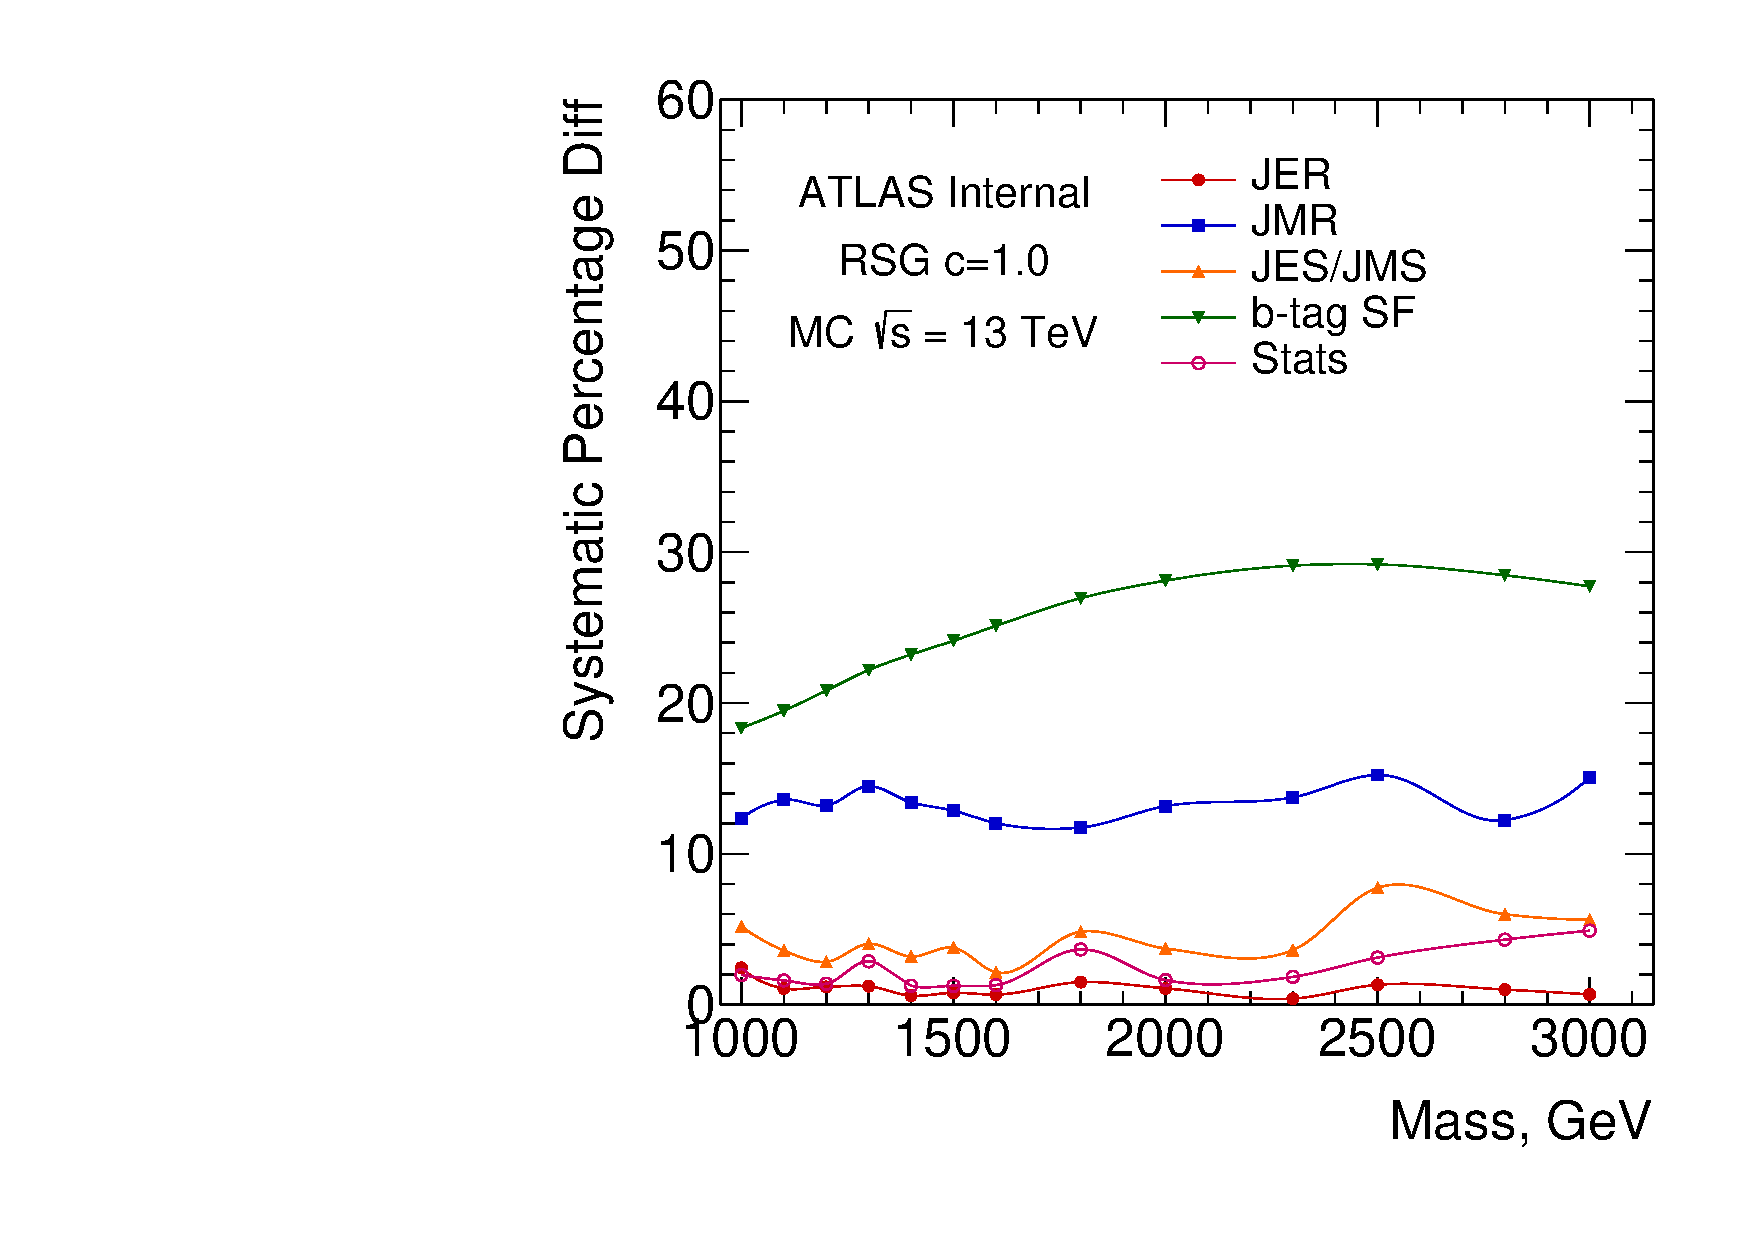
\includegraphics[width=\textwidth,angle=-90]{figures/boosted/Syst_MC/FourTag_RSG_syst.pdf}
        \caption{$4b$}
        \label{fig:signal_syst_summary-4b}
    \end{subfigure}
    \quad 
    \begin{subfigure}[b]{0.45\textwidth}
        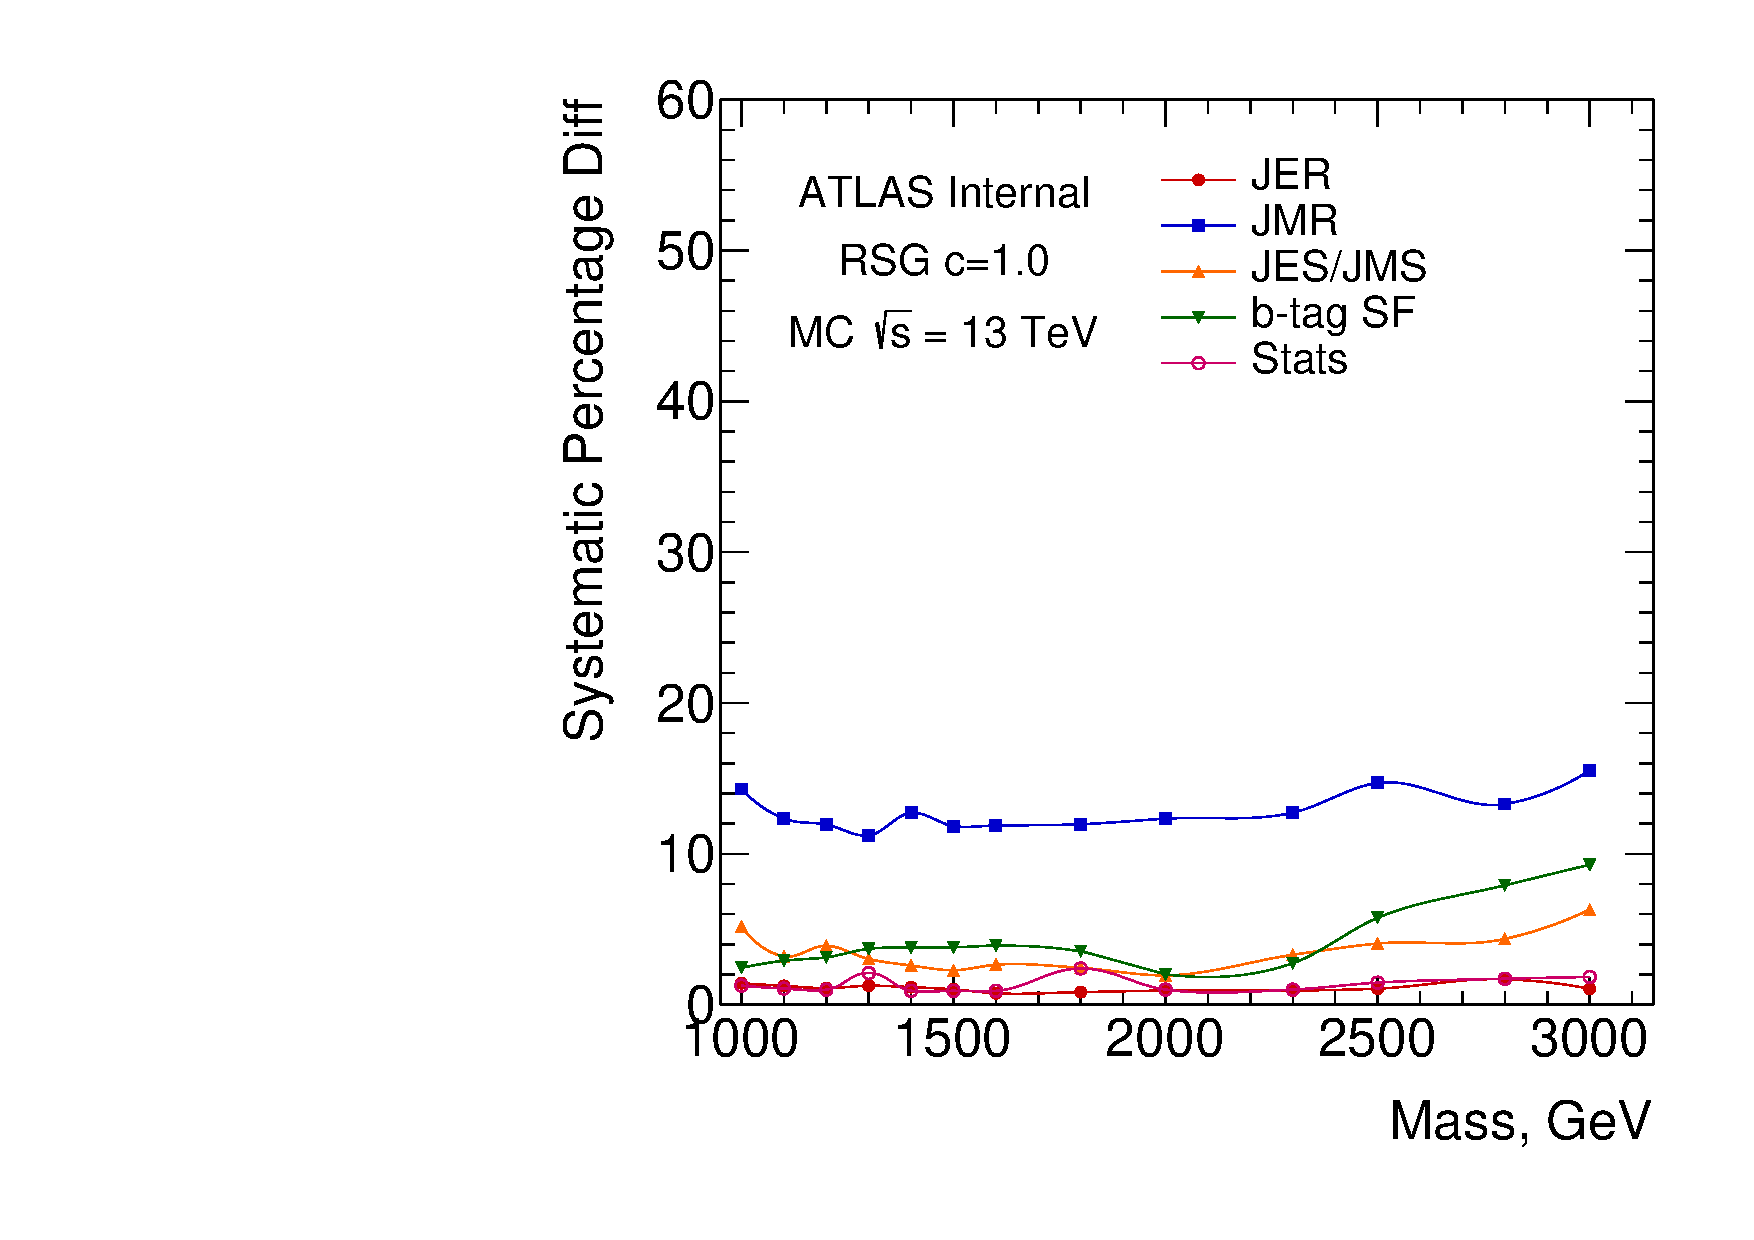
\includegraphics[width=\textwidth,angle=-90]{figures/boosted/Syst_MC/ThreeTag_RSG_syst.pdf}
        \caption{$3b$}
        \label{fig:signal_syst_summary-3b}
    \end{subfigure}
    \\
    \begin{subfigure}[b]{0.45\textwidth}
        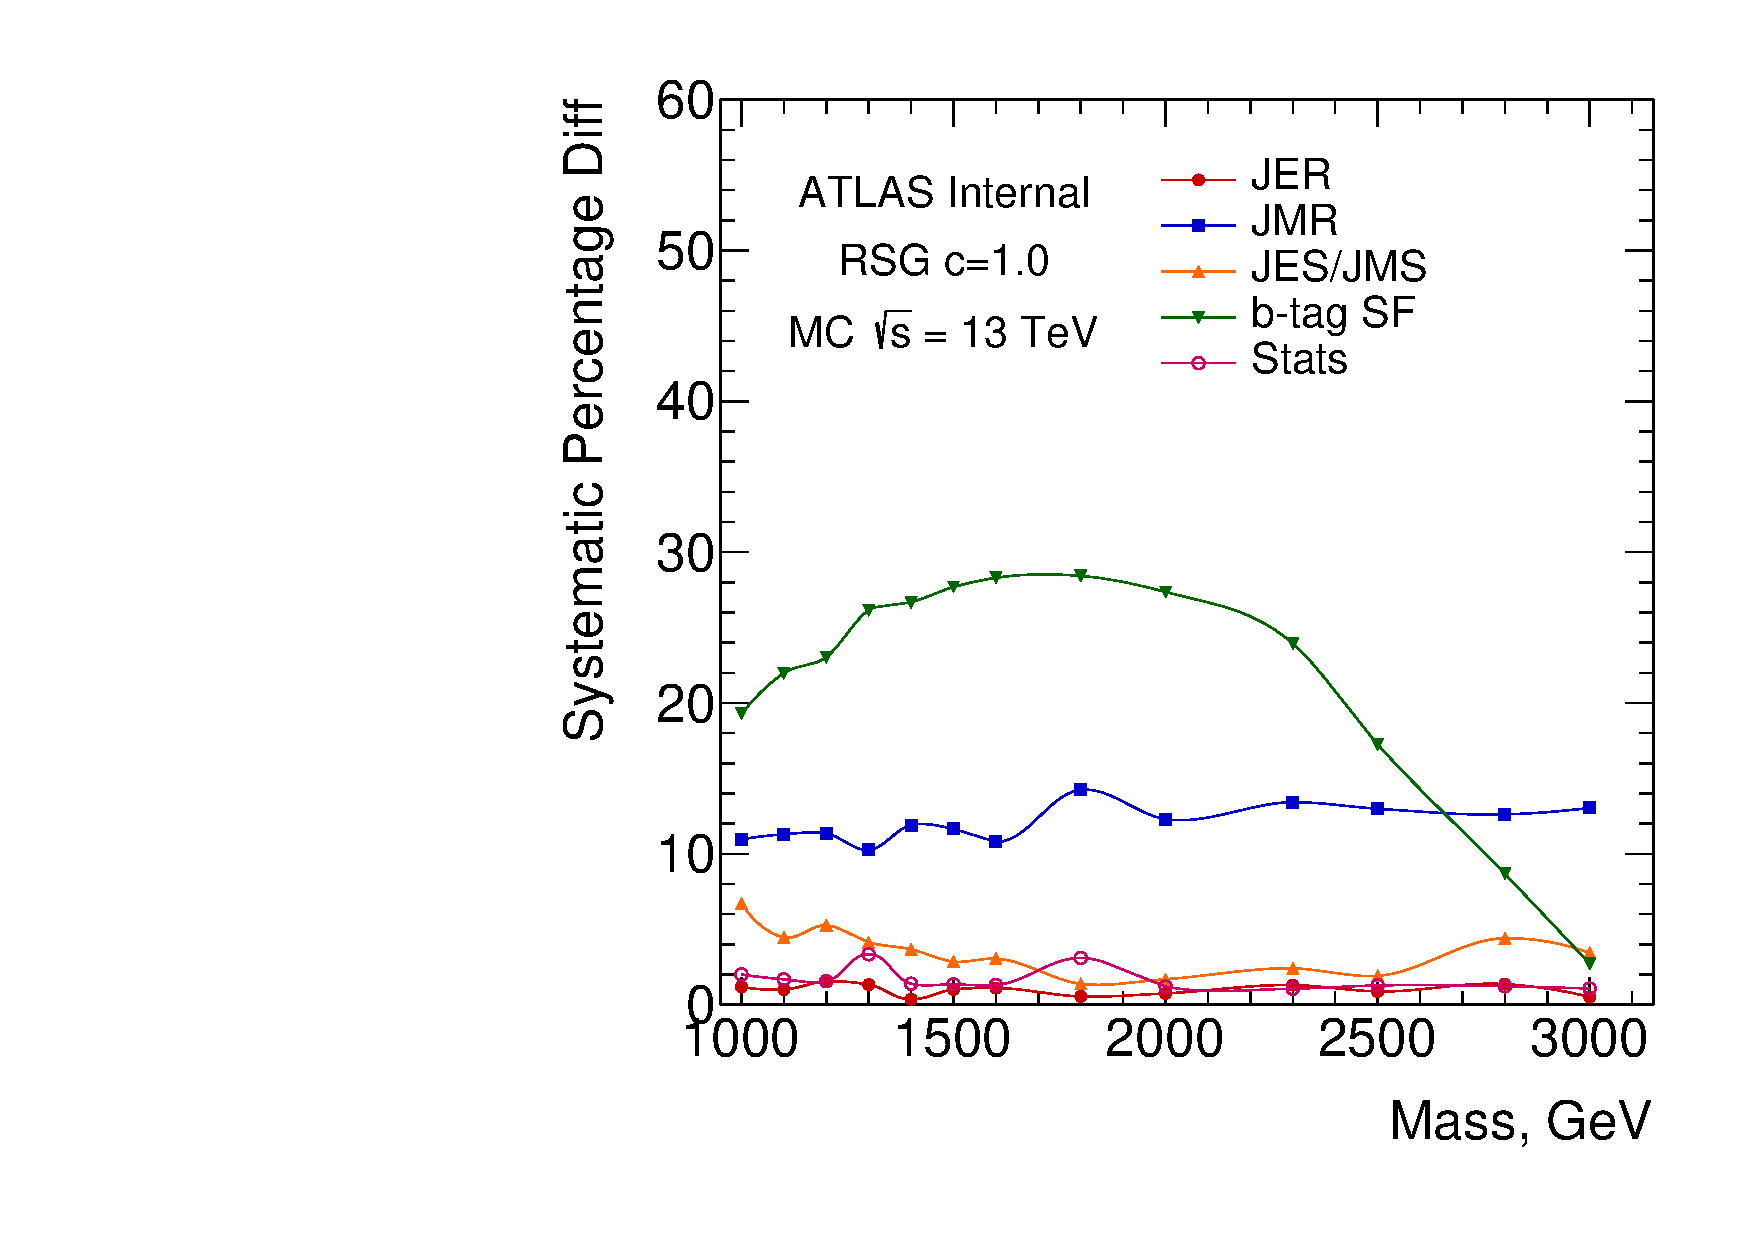
\includegraphics[width=\textwidth,angle=-90]{figures/boosted/Syst_MC/TwoTag_split_RSG_syst.pdf}
        \caption{$2bs$}
        \label{fig:signal_syst_summary-2b}
    \end{subfigure}
  \caption{Impact of each systematic on MC signal region prediction as a function of the \Grav~ mass.}
  \label{fig:signal_syst_summary}
\end{figure*}

\paragraph{}
The fractional size of systematics on MC as a function of the \Grav~ mass can be found in Figure~\ref{fig:signal_syst_summary}.
The largest uncertainty in the $4b$ and $2b$ channels comes from $b$-tagging, followed by the JMR uncertainty.
In the $3b$ channel, although $b$-tagging systematics is still one of the largest uncertainty categories, it is much smaller than in the $4b$ channel, as discussed in Section~\ref{sec:b-tagging-unc}. 


\begin{table}[htb!]
\begin{center}
\caption{Percent impact of the dominant systematics on the background acceptance
         and on the signal acceptance of \Grav~ with $c=1.0$ in the $4b$ channel signal region.}
\begin{footnotesize} 
\begin{tabular}{c|c|c|c|c|c|c} 
FourTag & totalbkg & qcd & ttbar & RSG1 1000 & RSG1 2000 & RSG1 3000 \\ 
\hline\hline 
JER & 0.45 & 0.27 & 3.98 & 2.44 & 1.07 & 0.67\\ 
JMR & 7.9 & 10.35 & 39.95 & 12.33 & 13.16 & 15.08\\ 
Top &  -  &  -  &  -  &  -  &  -  &  - \\ 
JES/JMS & 1.32 & 1.49 & 24.36 & 5.18 & 3.72 & 5.62\\ 
Bkg Est & 15.67 & 18.19 & 67.82 &  -  &  -  &  - \\ 
b-tag SF & 1.11 & 0.79 & 18.85 & 18.34 & 28.11 & 27.73\\ 
\hline 
Total Sys & 17.64 & 21.0 & 84.62 & 22.83 & 31.28 & 32.07\\ 
\hline 
Stat & 3.13 & 3.29 & 2.47 & 1.97 & 1.63 & 4.9\\ 
\hline 
Estimated Events & 34.59 & 32.91 & 1.68 & 10.07 & 0.25 & 0.0016\\ 
\hline\hline 
\end{tabular} 
\end{footnotesize} 
\newline 

\label{tab:summary-systematics-4b}
\end{center}
\end{table}

\begin{table}[htb!]
\begin{center}
\caption{Percent impact of the dominant systematics on the background acceptance
         and on the signal acceptance of \Grav~ with $c=1.0$ in the $3b$ channel signal region.}
\begin{footnotesize} 
\begin{tabular}{c|c|c|c|c|c|c} 
ThreeTag & totalbkg & qcd & ttbar & RSG1 1000 & RSG1 2000 & RSG1 3000 \\ 
\hline\hline 
JER & 1.38 & 3.52 & 17.5 & 1.41 & 0.93 & 1.08\\ 
JMR & 1.35 & 4.26 & 24.38 & 14.3 & 12.33 & 15.53\\ 
Top &  -  &  -  &  -  &  -  &  -  &  - \\ 
JES/JMS & 2.03 & 1.26 & 26.22 & 5.19 & 1.94 & 6.35\\ 
Bkg Est & 4.84 & 5.62 & 9.45 &  -  &  -  &  - \\ 
b-tag SF & 0.47 & 0.53 & 8.45 & 2.45 & 2.01 & 9.27\\ 
\hline 
Total Sys & 5.61 & 8.0 & 41.82 & 15.47 & 12.68 & 19.2\\ 
\hline 
Stat & 1.32 & 1.44 & 2.47 & 1.26 & 1.0 & 1.83\\ 
\hline 
Estimated Events & 780.89 & 701.52 & 79.38 & 26.0 & 0.76 & 0.013\\ 
\hline\hline 
\end{tabular} 
\end{footnotesize} 
\newline 

\label{tab:summary-systematics-3b}
\end{center}
\end{table}

\begin{table}[htb!]
\begin{center}
\caption{Percent impact of the dominant systematics on the background acceptance
         and on the signal acceptance of \Grav~ with $c=1.0$ in the $2bs$ channel signal region.}
\begin{footnotesize} 
\begin{tabular}{c|c|c|c|c|c|c} 
TwoTag split & totalbkg & qcd & ttbar & RSG1 1000 & RSG1 2000 & RSG1 3000 \\ 
\hline\hline 
JER & 0.25 & 0.48 & 3.14 & 1.18 & 0.74 & 0.5\\ 
JMR & 0.52 & 1.73 & 9.43 & 10.96 & 12.3 & 13.05\\ 
Top & 4.82 & 6.98 & 26.63 &  -  &  -  &  - \\ 
JES/JMS & 0.43 & 1.67 & 7.17 & 6.72 & 1.69 & 3.44\\ 
Bkg Est & 2.76 & 3.38 & 2.35 &  -  &  -  &  - \\ 
b-tag SF & 0.83 & 1.43 & 1.82 & 19.28 & 27.36 & 2.7\\ 
\hline 
Total Sys & 5.66 & 8.26 & 29.46 & 23.2 & 30.05 & 13.77\\ 
\hline 
Stat & 0.6 & 0.42 & 2.48 & 2.0 & 1.2 & 1.07\\ 
\hline 
Estimated Events & 4252.44 & 3393.74 & 858.7 & 10.87 & 0.6 & 0.039\\ 
\hline\hline 
\end{tabular} 
\end{footnotesize} 
\newline 

\label{tab:summary-systematics-2b}
\end{center}
\end{table}


% \paragraph{}
% The final background prediction of scaled \mtwoJ along with total uncertainties can be found in Figure~\ref{fig:FinalBkg_sys-4b-pole}, ~\ref{fig:FinalBkg_sys-3b-pole}, and ~\ref{fig:FinalBkg_sys-2b-pole}.

% \begin{figure}
% \begin{center}
% 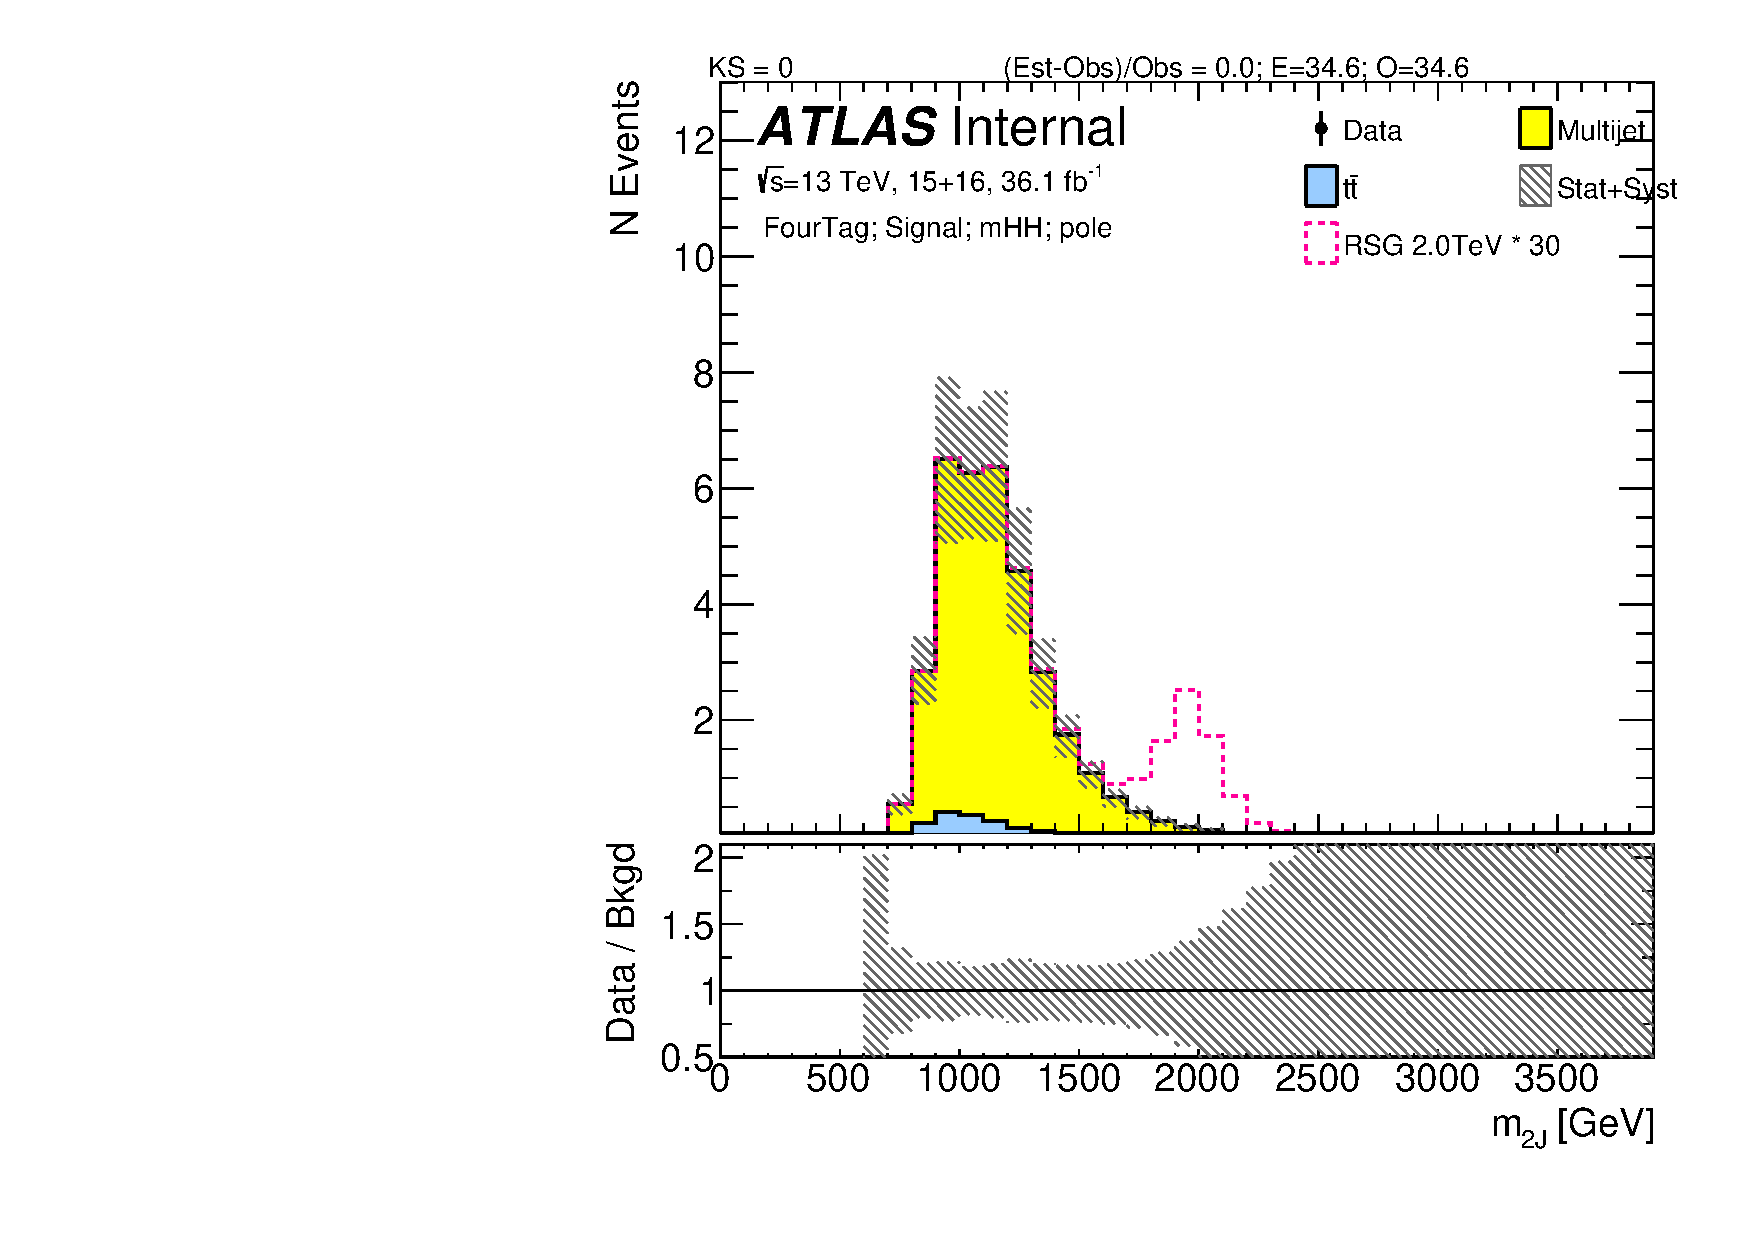
\includegraphics[width=0.48\textwidth,angle=-90]{figures/boosted/Signal_Syst/Moriond_bkg_9_FourTag_Signal_mHH_pole_blind.pdf}
% 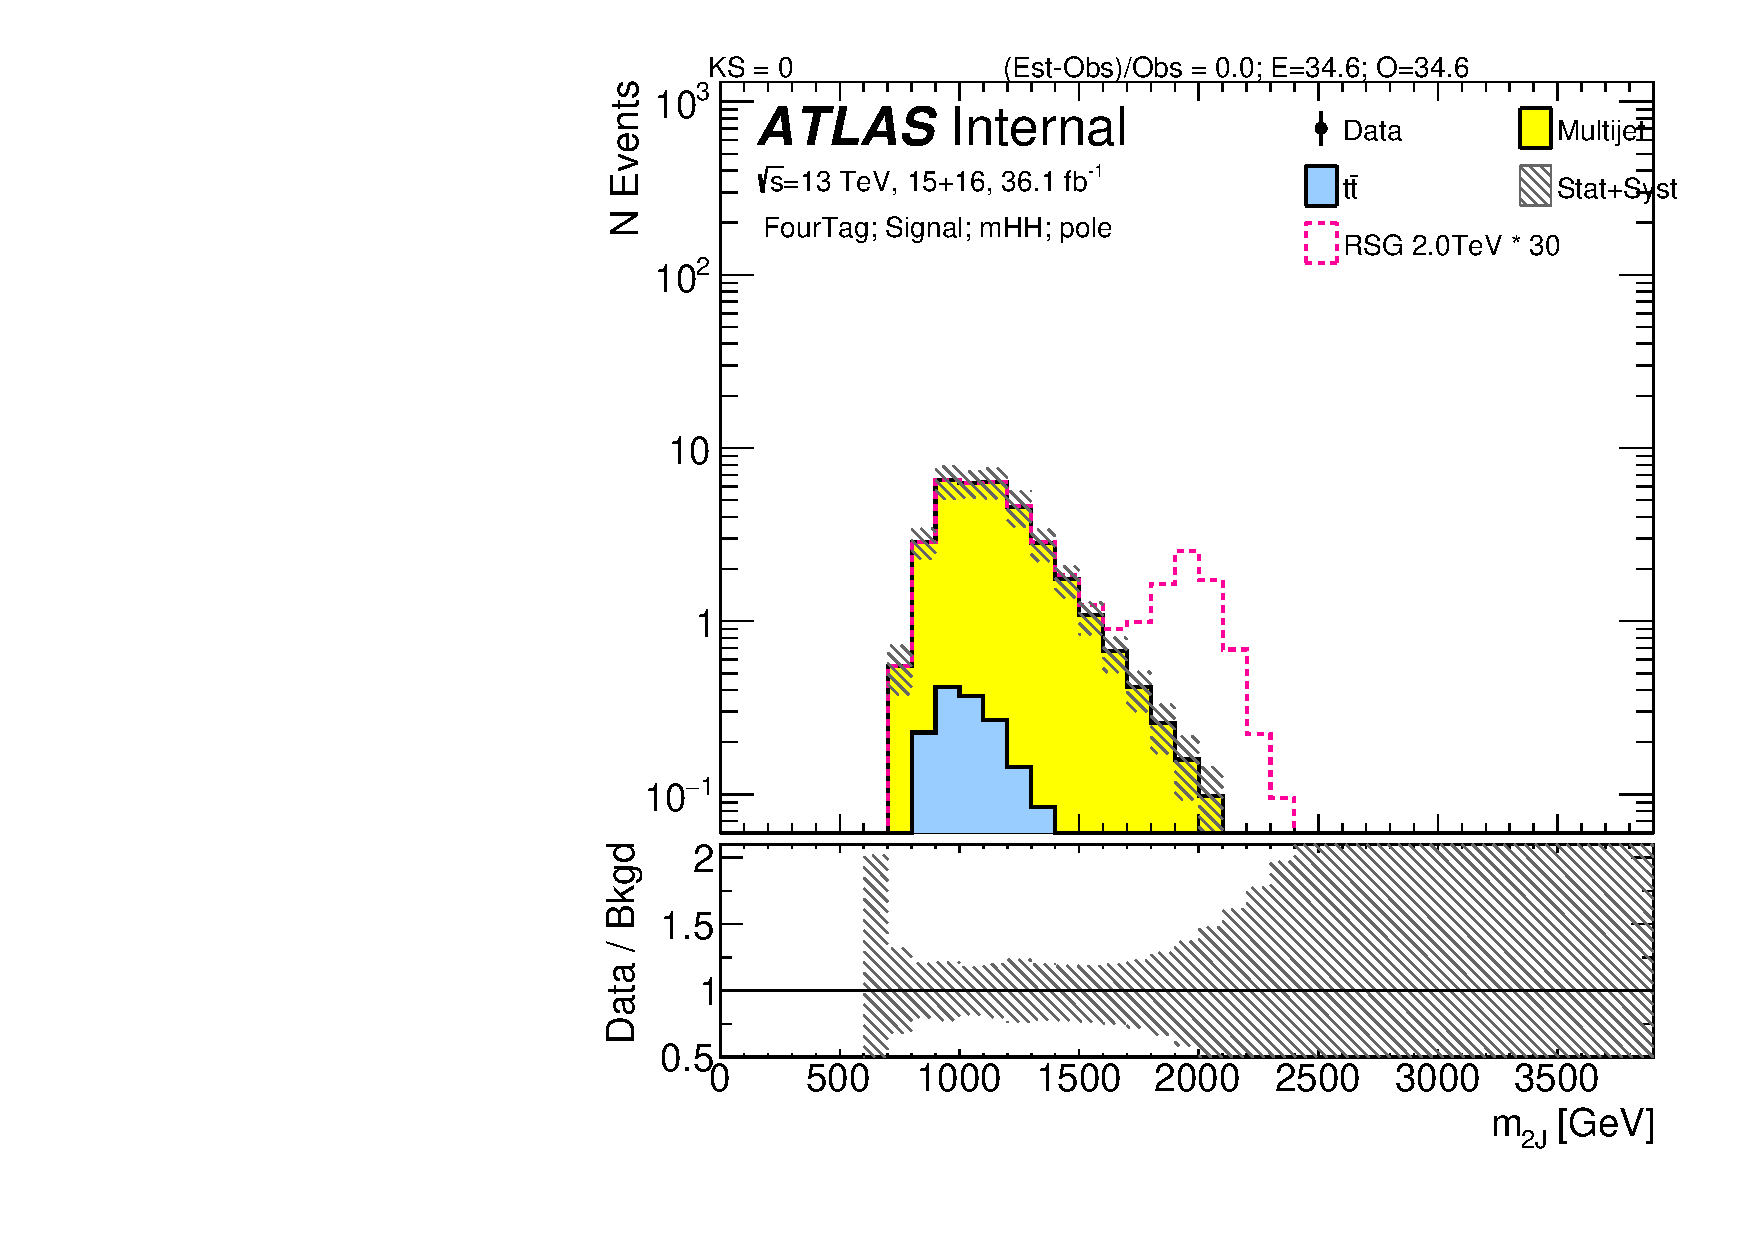
\includegraphics[width=0.48\textwidth,angle=-90]{figures/boosted/Signal_Syst/Moriond_bkg_9_FourTag_Signal_mHH_pole_1_blind.pdf}
% \caption{The total background estimation in $4b$ signal region, scaled mJJ, with linear scale on the left and with log scale on the right, along with total uncertainties (stats.$+$systematic) variation up and down.}
% \label{fig:FinalBkg_sys-4b-pole}
% \end{center}
% \end{figure}


% \begin{figure}
% \begin{center}
% 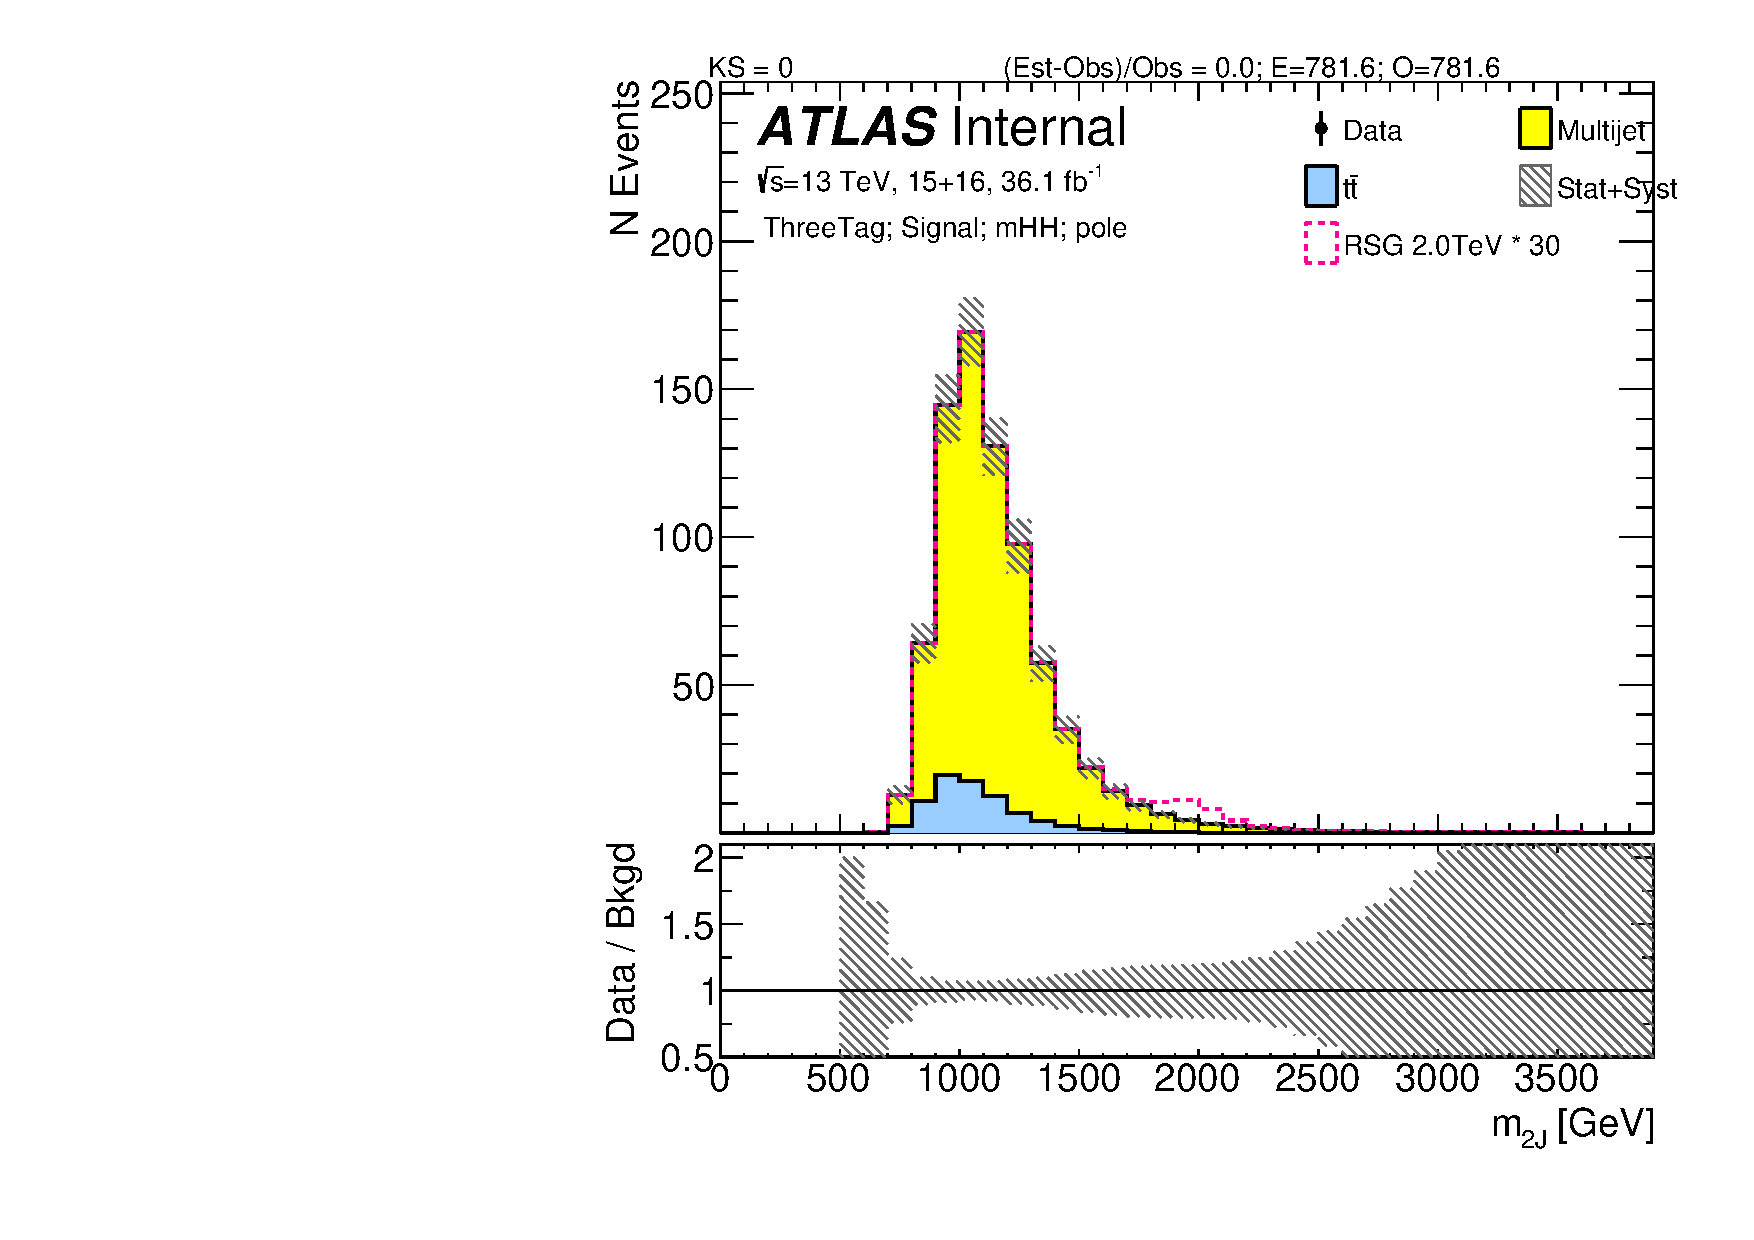
\includegraphics[width=0.48\textwidth,angle=-90]{figures/boosted/Signal_Syst/Moriond_bkg_9_ThreeTag_Signal_mHH_pole_blind.pdf}
% 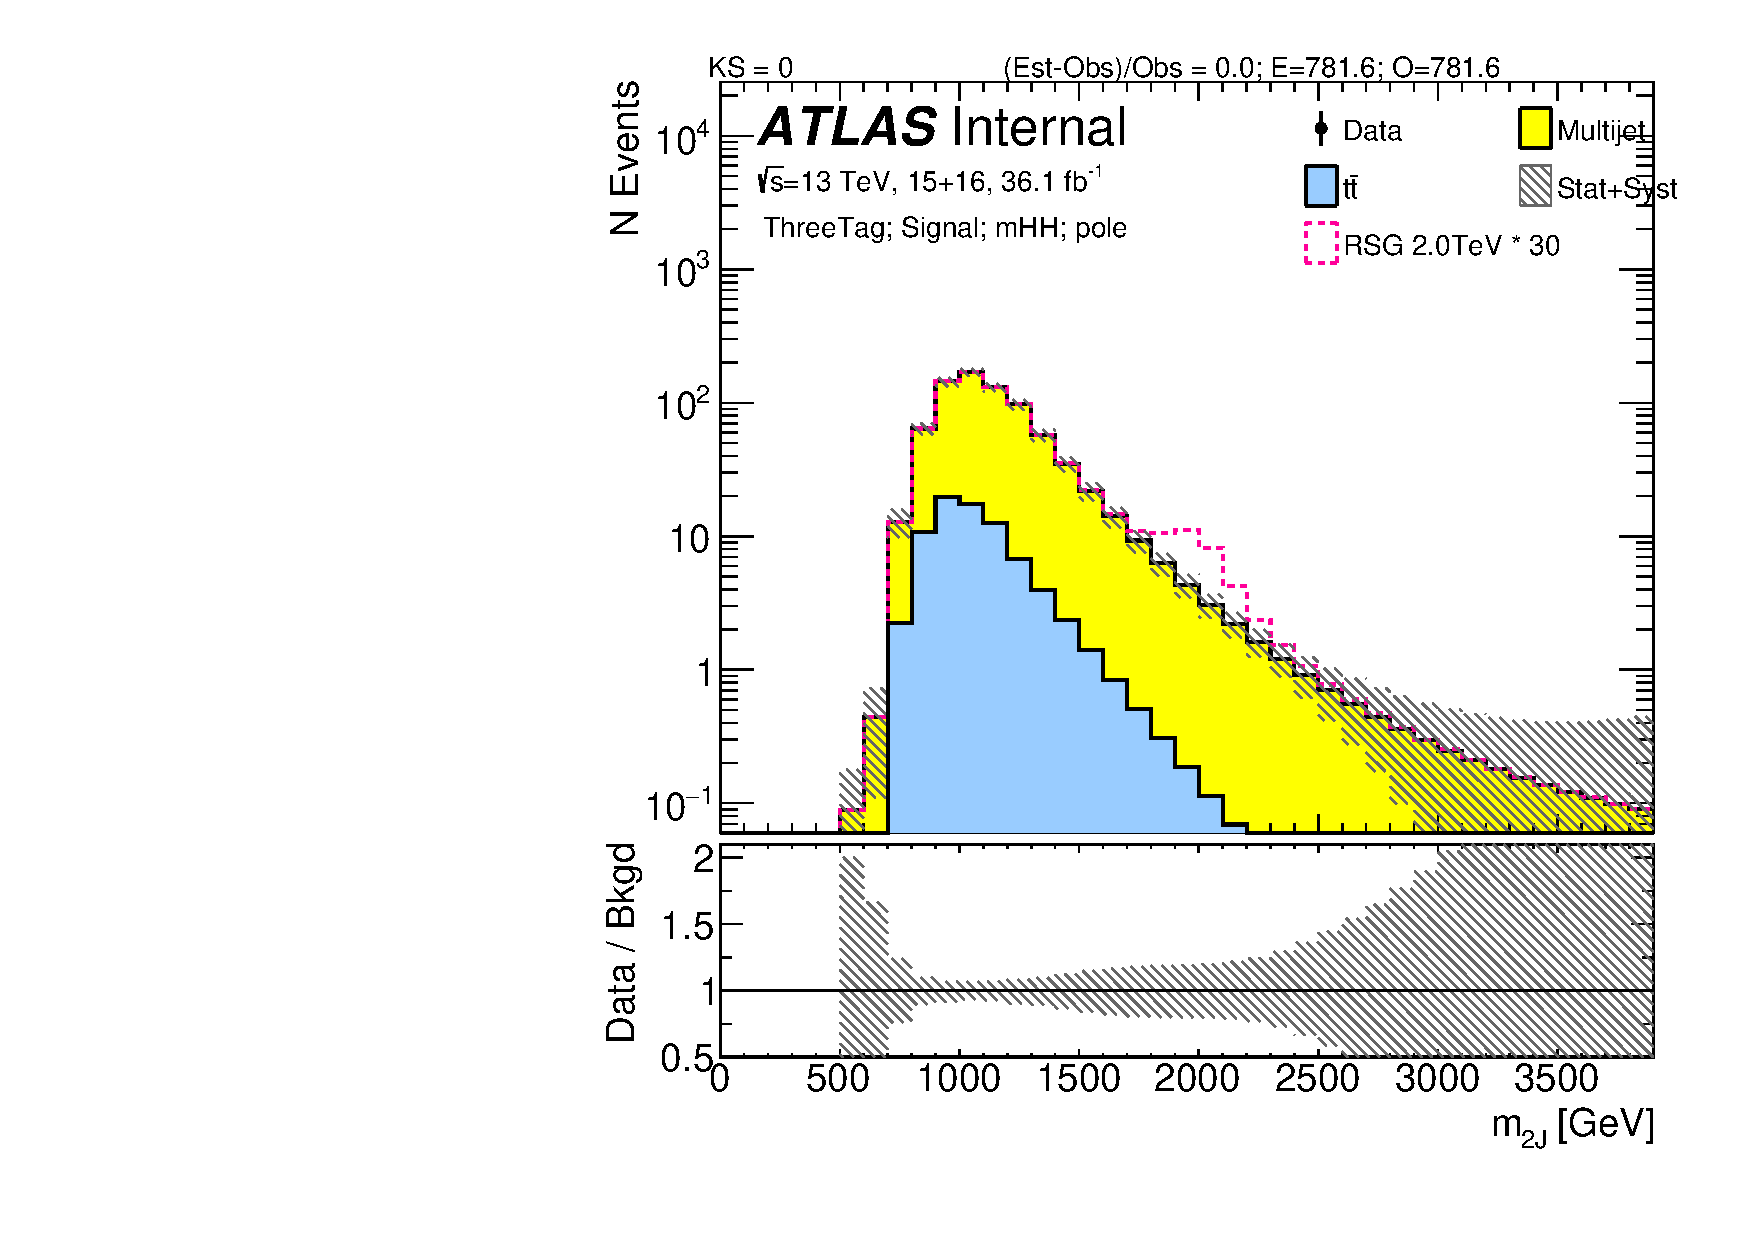
\includegraphics[width=0.48\textwidth,angle=-90]{figures/boosted/Signal_Syst/Moriond_bkg_9_ThreeTag_Signal_mHH_pole_1_blind.pdf}
% \caption{The total background estimation in $3b$ signal region, scaled mJJ, with linear scale on the left and with log scale on the right, along with total uncertainties (stats.$+$systematic) variation up and down.}
% \label{fig:FinalBkg_sys-3b-pole}
% \end{center}
% \end{figure}


% \begin{figure}
% \begin{center}
% 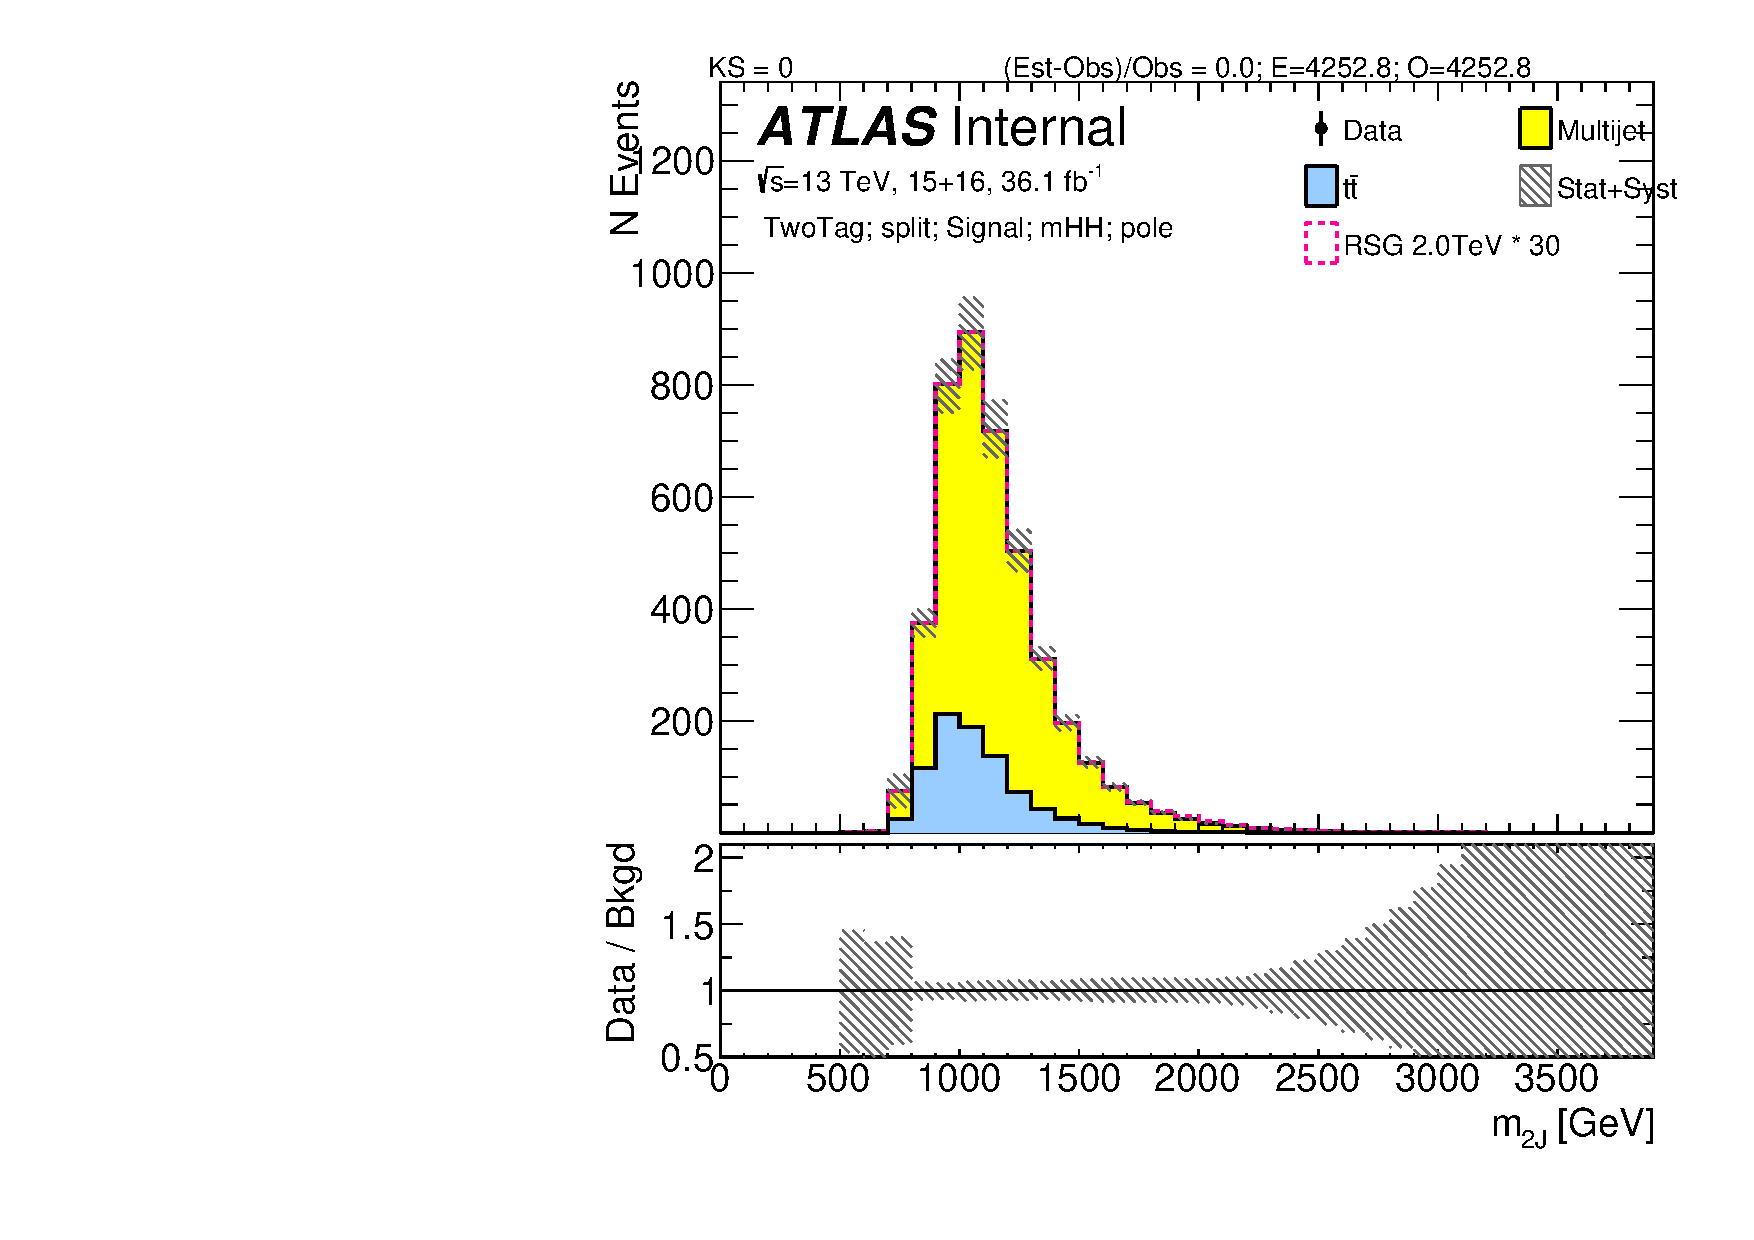
\includegraphics[width=0.48\textwidth,angle=-90]{figures/boosted/Signal_Syst/Moriond_bkg_9_TwoTag_split_Signal_mHH_pole_blind.pdf}
% 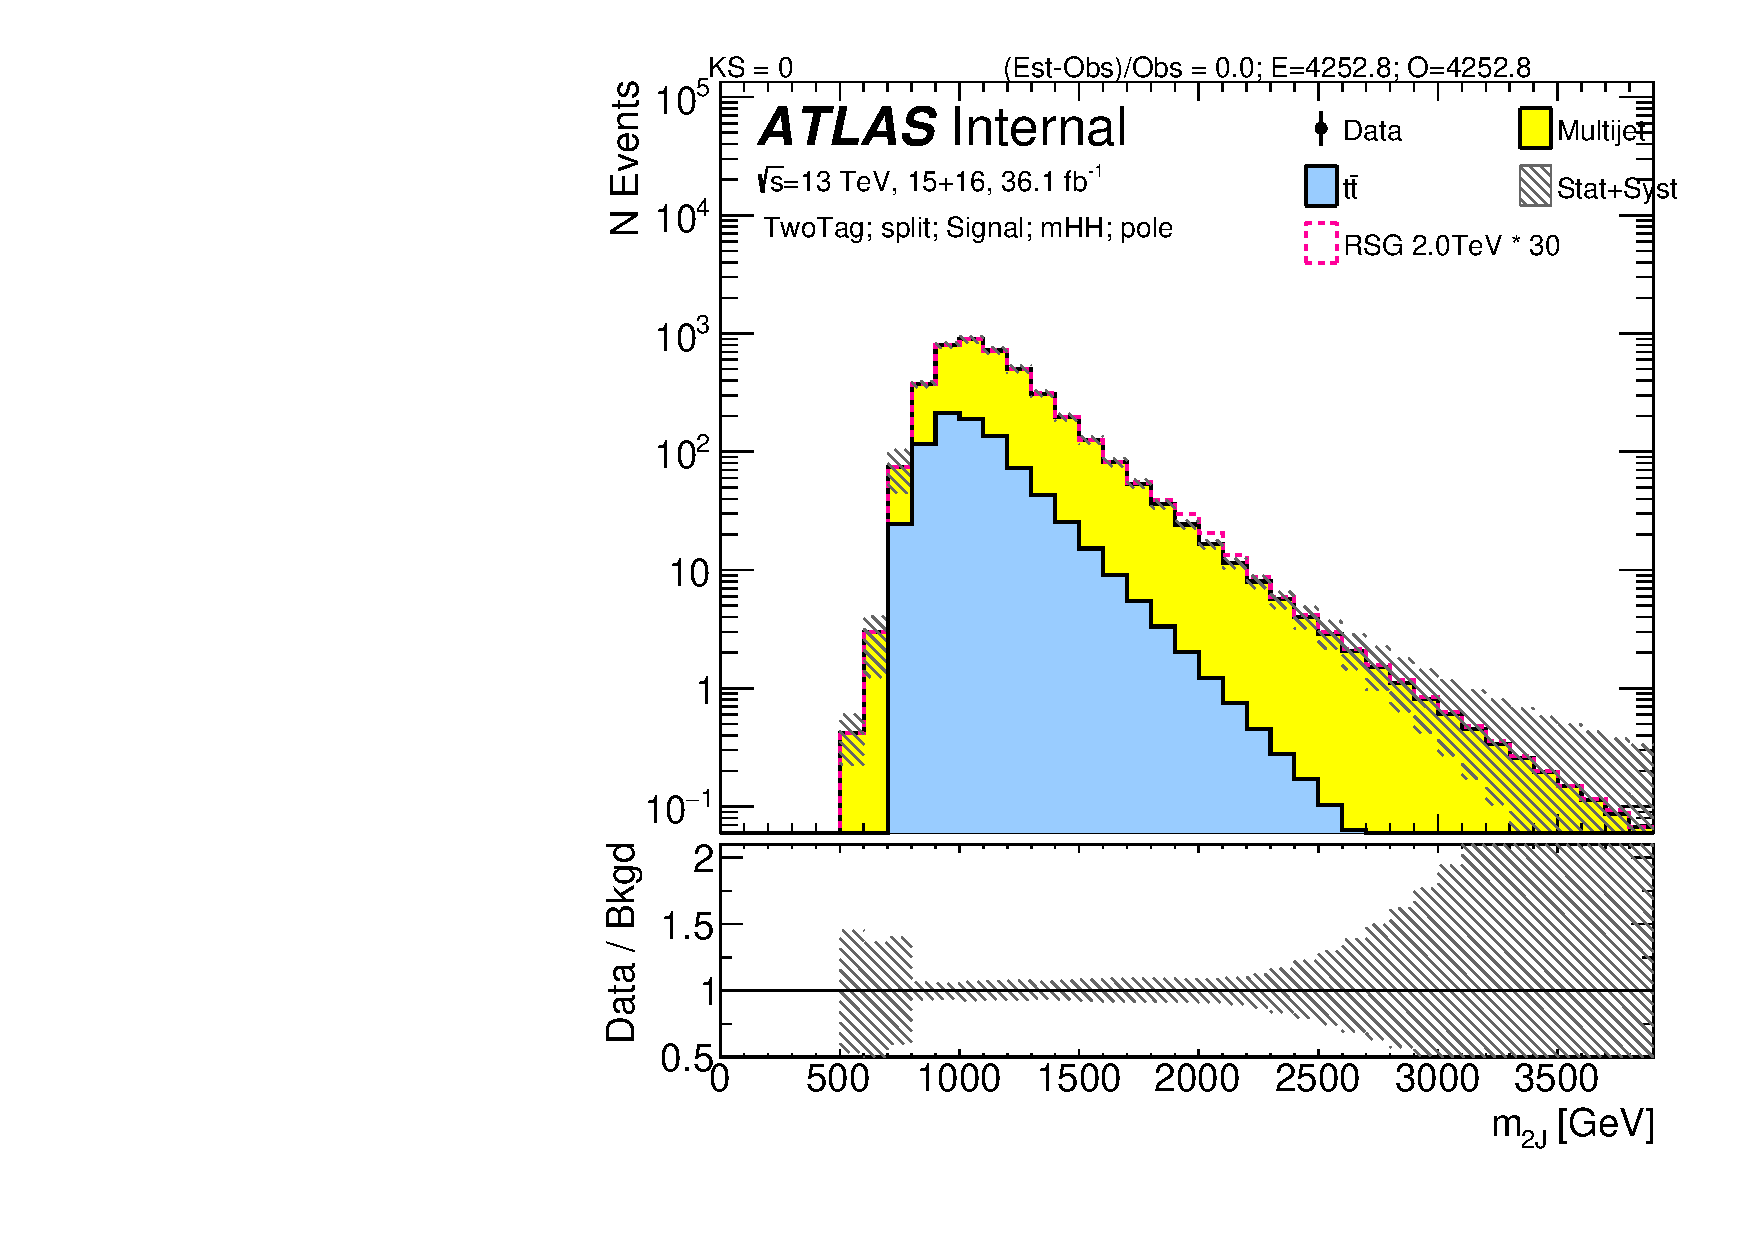
\includegraphics[width=0.48\textwidth,angle=-90]{figures/boosted/Signal_Syst/Moriond_bkg_9_TwoTag_split_Signal_mHH_pole_1_blind.pdf}
% \caption{The total background estimation in $2bs$ signal region, scaled mJJ, with linear scale on the left and with log scale on the right, along with total uncertainties (stats.$+$systematic) variation up and down.}
% \label{fig:FinalBkg_sys-2b-pole}
% \end{center}
% \end{figure}


%%%%%%%%%%%%%%%%%%%%%%%%%%%%%%%%%%%%%%%%%%%%%%%%%%%%%%%%%%%%%%%%%%%%%%%
%%%%%%%%%%%%%%%%%%%%%%%%%%%%%%%%%%%%%%%%%%%%%%%%%%%%%%%%%%%%%%%%%%%%%%%